\documentclass[twoside]{book}

% Packages required by doxygen
\usepackage{fixltx2e}
\usepackage{calc}
\usepackage{doxygen}
\usepackage[export]{adjustbox} % also loads graphicx
\usepackage{graphicx}
\usepackage[utf8]{inputenc}
\usepackage{makeidx}
\usepackage{multicol}
\usepackage{multirow}
\PassOptionsToPackage{warn}{textcomp}
\usepackage{textcomp}
\usepackage[nointegrals]{wasysym}
\usepackage[table]{xcolor}

% Font selection
\usepackage[T1]{fontenc}
\usepackage[scaled=.90]{helvet}
\usepackage{courier}
\usepackage{amssymb}
\usepackage{sectsty}
\renewcommand{\familydefault}{\sfdefault}
\allsectionsfont{%
  \fontseries{bc}\selectfont%
  \color{darkgray}%
}
\renewcommand{\DoxyLabelFont}{%
  \fontseries{bc}\selectfont%
  \color{darkgray}%
}
\newcommand{\+}{\discretionary{\mbox{\scriptsize$\hookleftarrow$}}{}{}}

% Page & text layout
\usepackage{geometry}
\geometry{%
  a4paper,%
  top=2.5cm,%
  bottom=2.5cm,%
  left=2.5cm,%
  right=2.5cm%
}
\tolerance=750
\hfuzz=15pt
\hbadness=750
\setlength{\emergencystretch}{15pt}
\setlength{\parindent}{0cm}
\setlength{\parskip}{3ex plus 2ex minus 2ex}
\makeatletter
\renewcommand{\paragraph}{%
  \@startsection{paragraph}{4}{0ex}{-1.0ex}{1.0ex}{%
    \normalfont\normalsize\bfseries\SS@parafont%
  }%
}
\renewcommand{\subparagraph}{%
  \@startsection{subparagraph}{5}{0ex}{-1.0ex}{1.0ex}{%
    \normalfont\normalsize\bfseries\SS@subparafont%
  }%
}
\makeatother

% Headers & footers
\usepackage{fancyhdr}
\pagestyle{fancyplain}
\fancyhead[LE]{\fancyplain{}{\bfseries\thepage}}
\fancyhead[CE]{\fancyplain{}{}}
\fancyhead[RE]{\fancyplain{}{\bfseries\leftmark}}
\fancyhead[LO]{\fancyplain{}{\bfseries\rightmark}}
\fancyhead[CO]{\fancyplain{}{}}
\fancyhead[RO]{\fancyplain{}{\bfseries\thepage}}
\fancyfoot[LE]{\fancyplain{}{}}
\fancyfoot[CE]{\fancyplain{}{}}
\fancyfoot[RE]{\fancyplain{}{\bfseries\scriptsize Generated by Doxygen }}
\fancyfoot[LO]{\fancyplain{}{\bfseries\scriptsize Generated by Doxygen }}
\fancyfoot[CO]{\fancyplain{}{}}
\fancyfoot[RO]{\fancyplain{}{}}
\renewcommand{\footrulewidth}{0.4pt}
\renewcommand{\chaptermark}[1]{%
  \markboth{#1}{}%
}
\renewcommand{\sectionmark}[1]{%
  \markright{\thesection\ #1}%
}

% Indices & bibliography
\usepackage{natbib}
\usepackage[titles]{tocloft}
\setcounter{tocdepth}{3}
\setcounter{secnumdepth}{5}
\makeindex

% Hyperlinks (required, but should be loaded last)
\usepackage{ifpdf}
\ifpdf
  \usepackage[pdftex,pagebackref=true]{hyperref}
\else
  \usepackage[ps2pdf,pagebackref=true]{hyperref}
\fi
\hypersetup{%
  colorlinks=true,%
  linkcolor=blue,%
  citecolor=blue,%
  unicode%
}

% Custom commands
\newcommand{\clearemptydoublepage}{%
  \newpage{\pagestyle{empty}\cleardoublepage}%
}

\usepackage{caption}
\captionsetup{labelsep=space,justification=centering,font={bf},singlelinecheck=off,skip=4pt,position=top}

%===== C O N T E N T S =====

\begin{document}

% Titlepage & ToC
\hypersetup{pageanchor=false,
             bookmarksnumbered=true,
             pdfencoding=unicode
            }
\pagenumbering{alph}
\begin{titlepage}
\vspace*{7cm}
\begin{center}%
{\Large My Project }\\
\vspace*{1cm}
{\large Generated by Doxygen 1.8.13}\\
\end{center}
\end{titlepage}
\clearemptydoublepage
\pagenumbering{roman}
\tableofcontents
\clearemptydoublepage
\pagenumbering{arabic}
\hypersetup{pageanchor=true}

%--- Begin generated contents ---
\chapter{File Index}
\section{File List}
Here is a list of all files with brief descriptions\+:\begin{DoxyCompactList}
\item\contentsline{section}{\hyperlink{main_8c}{main.\+c} }{\pageref{main_8c}}{}
\item\contentsline{section}{\hyperlink{utils_8c}{utils.\+c} }{\pageref{utils_8c}}{}
\item\contentsline{section}{\hyperlink{utils_8h}{utils.\+h} }{\pageref{utils_8h}}{}
\end{DoxyCompactList}

\chapter{File Documentation}
\hypertarget{main_8c}{}\section{main.\+c File Reference}
\label{main_8c}\index{main.\+c@{main.\+c}}
{\ttfamily \#include $<$stdio.\+h$>$}\newline
{\ttfamily \#include $<$stdlib.\+h$>$}\newline
{\ttfamily \#include $<$string.\+h$>$}\newline
{\ttfamily \#include $<$time.\+h$>$}\newline
{\ttfamily \#include $<$unistd.\+h$>$}\newline
{\ttfamily \#include \char`\"{}utils.\+h\char`\"{}}\newline
Include dependency graph for main.\+c\+:
\nopagebreak
\begin{figure}[H]
\begin{center}
\leavevmode
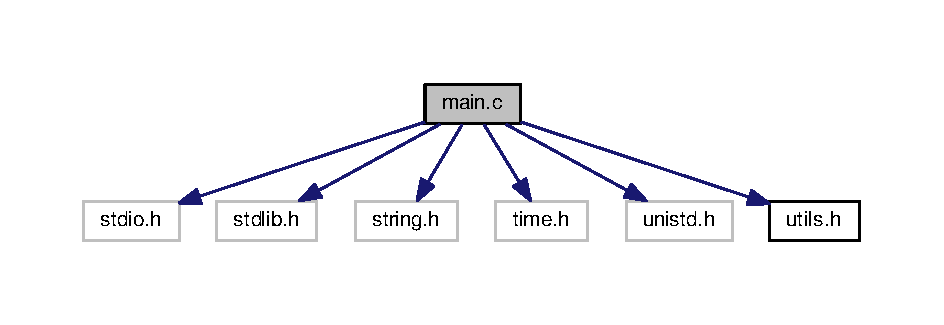
\includegraphics[width=350pt]{main_8c__incl}
\end{center}
\end{figure}
\subsection*{Macros}
\begin{DoxyCompactItemize}
\item 
\#define \hyperlink{main_8c_a70ed59adcb4159ac551058053e649640}{S\+I\+ZE}~10
\end{DoxyCompactItemize}
\subsection*{Functions}
\begin{DoxyCompactItemize}
\item 
void \hyperlink{main_8c_a8ff4ae8bd48d4716785cd92d70deda7b}{run} (int is\+Pv\+C\+OM)
\item 
int \hyperlink{main_8c_ae66f6b31b5ad750f1fe042a706a4e3d4}{main} ()
\end{DoxyCompactItemize}


\subsection{Macro Definition Documentation}
\mbox{\Hypertarget{main_8c_a70ed59adcb4159ac551058053e649640}\label{main_8c_a70ed59adcb4159ac551058053e649640}} 
\index{main.\+c@{main.\+c}!S\+I\+ZE@{S\+I\+ZE}}
\index{S\+I\+ZE@{S\+I\+ZE}!main.\+c@{main.\+c}}
\subsubsection{\texorpdfstring{S\+I\+ZE}{SIZE}}
{\footnotesize\ttfamily \#define S\+I\+ZE~10}



Definition at line 17 of file main.\+c.



\subsection{Function Documentation}
\mbox{\Hypertarget{main_8c_ae66f6b31b5ad750f1fe042a706a4e3d4}\label{main_8c_ae66f6b31b5ad750f1fe042a706a4e3d4}} 
\index{main.\+c@{main.\+c}!main@{main}}
\index{main@{main}!main.\+c@{main.\+c}}
\subsubsection{\texorpdfstring{main()}{main()}}
{\footnotesize\ttfamily int main (\begin{DoxyParamCaption}{ }\end{DoxyParamCaption})}



Definition at line 131 of file main.\+c.


\begin{DoxyCode}
131           \{
132     \hyperlink{utils_8c_a9d7e8af417b6d543da691e9c0e2f6f9f}{clearScreen}();
133     \hyperlink{utils_8c_a1ea6231221c4e03a66d89d0c38aa71cc}{printBattleship}();
134     \hyperlink{utils_8c_a087a2b7743093438ffebaedb708e3283}{printMenu1}();
135 
136     \textcolor{keywordtype}{char} optionMenu1;
137     \textcolor{keywordtype}{char} optionMenu2;
138 
139     \textcolor{keywordflow}{do}\{
140         scanf(\textcolor{stringliteral}{" %c"}, &optionMenu1);
141         \textcolor{keywordflow}{switch}(optionMenu1)\{
142             \textcolor{keywordflow}{case} \textcolor{charliteral}{'1'}:
143                 \hyperlink{utils_8c_a9d7e8af417b6d543da691e9c0e2f6f9f}{clearScreen}();
144                 \hyperlink{utils_8c_a1ea6231221c4e03a66d89d0c38aa71cc}{printBattleship}();
145                 \hyperlink{utils_8c_a4f2acb39a12d6c7570980ae92ec9befc}{printMenu2}();
146 
147                 \textcolor{keywordflow}{do}\{
148                     scanf(\textcolor{stringliteral}{" %c"}, &optionMenu2);
149                     \textcolor{keywordflow}{switch}(optionMenu2)\{
150                         \textcolor{keywordflow}{case} \textcolor{charliteral}{'1'}:
151                             \hyperlink{utils_8c_a9d7e8af417b6d543da691e9c0e2f6f9f}{clearScreen}();
152                             \hyperlink{utils_8c_a1ea6231221c4e03a66d89d0c38aa71cc}{printBattleship}();
153                             printf(\textcolor{stringliteral}{"\(\backslash\)n\(\backslash\)nBem-vindo à opção de jogo PvCOM!\(\backslash\)n\(\backslash\)n\(\backslash\)n"});
154                             \hyperlink{main_8c_a8ff4ae8bd48d4716785cd92d70deda7b}{run}(1);
155                             \hyperlink{utils_8c_a9d7e8af417b6d543da691e9c0e2f6f9f}{clearScreen}();
156                             \hyperlink{utils_8c_a1ea6231221c4e03a66d89d0c38aa71cc}{printBattleship}();
157                             \hyperlink{utils_8c_a4f2acb39a12d6c7570980ae92ec9befc}{printMenu2}();
158                             \textcolor{keywordflow}{break};
159                         \textcolor{keywordflow}{case} \textcolor{charliteral}{'2'}:
160                             \hyperlink{utils_8c_a9d7e8af417b6d543da691e9c0e2f6f9f}{clearScreen}();
161                             \hyperlink{utils_8c_a1ea6231221c4e03a66d89d0c38aa71cc}{printBattleship}();
162                             printf(\textcolor{stringliteral}{"\(\backslash\)n\(\backslash\)nBem-vindo à opção de jogo PvP!\(\backslash\)n\(\backslash\)n\(\backslash\)n"});
163                             \hyperlink{main_8c_a8ff4ae8bd48d4716785cd92d70deda7b}{run}(0);
164                             \hyperlink{utils_8c_a9d7e8af417b6d543da691e9c0e2f6f9f}{clearScreen}();
165                             \hyperlink{utils_8c_a1ea6231221c4e03a66d89d0c38aa71cc}{printBattleship}();
166                             \hyperlink{utils_8c_a4f2acb39a12d6c7570980ae92ec9befc}{printMenu2}();
167                             \textcolor{keywordflow}{break};
168                         \textcolor{keywordflow}{case} \textcolor{charliteral}{'3'}:\textcolor{keywordflow}{break};
169                         \textcolor{keywordflow}{default}:
170                             printf(\textcolor{stringliteral}{"Opção de menu inválida!\(\backslash\)n"});
171                     \}
172 
173                 \}\textcolor{keywordflow}{while}((optionMenu2)!= \textcolor{charliteral}{'2'});
174 
175                 \hyperlink{utils_8c_a9d7e8af417b6d543da691e9c0e2f6f9f}{clearScreen}();
176                 \hyperlink{utils_8c_a1ea6231221c4e03a66d89d0c38aa71cc}{printBattleship}();
177                 \hyperlink{utils_8c_a087a2b7743093438ffebaedb708e3283}{printMenu1}();
178                 \textcolor{keywordflow}{break};
179             \textcolor{keywordflow}{case} \textcolor{charliteral}{'2'}:
180                 \hyperlink{utils_8c_a9d7e8af417b6d543da691e9c0e2f6f9f}{clearScreen}();
181                 \hyperlink{utils_8c_a1ea6231221c4e03a66d89d0c38aa71cc}{printBattleship}();
182                 \hyperlink{utils_8c_a4898a09411ad503295bdbe640b05dd10}{printAbout}();
183                 \hyperlink{utils_8c_a087a2b7743093438ffebaedb708e3283}{printMenu1}();
184                 \textcolor{keywordflow}{break};
185             \textcolor{keywordflow}{case} \textcolor{charliteral}{'3'}: \textcolor{keywordflow}{break};
186             \textcolor{keywordflow}{default}:
187                 printf(\textcolor{stringliteral}{"Opção de menu inválida!\(\backslash\)n"});
188         \}
189     \}\textcolor{keywordflow}{while}((optionMenu1 = getchar())!= \textcolor{charliteral}{'3'});
190 
191     \textcolor{keywordflow}{return}(0);
192 \}
\end{DoxyCode}
\mbox{\Hypertarget{main_8c_a8ff4ae8bd48d4716785cd92d70deda7b}\label{main_8c_a8ff4ae8bd48d4716785cd92d70deda7b}} 
\index{main.\+c@{main.\+c}!run@{run}}
\index{run@{run}!main.\+c@{main.\+c}}
\subsubsection{\texorpdfstring{run()}{run()}}
{\footnotesize\ttfamily void run (\begin{DoxyParamCaption}\item[{int}]{is\+Pv\+C\+OM }\end{DoxyParamCaption})}

Executa o jogo com as opções\+: 0 se deseja jogar PvP, 1 se deseja jogar Pv\+C\+OM


\begin{DoxyParams}{Parameters}
{\em is\+Pv\+C\+OM} & Defini o tipo de jogo\+: 0 PvP ou 1 Pv\+C\+OM \\
\hline
\end{DoxyParams}


Definition at line 24 of file main.\+c.


\begin{DoxyCode}
24                      \{
25     \textcolor{keywordflow}{while}(1)\{
26         \textcolor{comment}{// inicio o tabuleiro para o primeiro jogador}
27         \textcolor{keywordtype}{char} tabuleiro1[\hyperlink{main_8c_a70ed59adcb4159ac551058053e649640}{SIZE}][\hyperlink{main_8c_a70ed59adcb4159ac551058053e649640}{SIZE}];
28         \textcolor{keywordtype}{char} jogadas1[\hyperlink{main_8c_a70ed59adcb4159ac551058053e649640}{SIZE}][\hyperlink{main_8c_a70ed59adcb4159ac551058053e649640}{SIZE}];
29         \textcolor{keywordtype}{char} nomeJogador1[100];
30 
31         printf(\textcolor{stringliteral}{"Jogador 1, informe o seu nome: "});
32         scanf(\textcolor{stringliteral}{"%s"}, nomeJogador1);
33         \hyperlink{utils_8c_a821efd1de9257a6ac8bce69ecc1e5dfc}{initMatrix}(jogadas1);
34         \hyperlink{utils_8c_a8dbfb8ff4e945c557e1baa84ca1c39fa}{putShips}(nomeJogador1, tabuleiro1);
35 
36         \textcolor{comment}{// inicio o tabuleiro para o segundo jogador}
37         \textcolor{keywordtype}{char} tabuleiro2[\hyperlink{main_8c_a70ed59adcb4159ac551058053e649640}{SIZE}][\hyperlink{main_8c_a70ed59adcb4159ac551058053e649640}{SIZE}];
38         \textcolor{keywordtype}{char} jogadas2[\hyperlink{main_8c_a70ed59adcb4159ac551058053e649640}{SIZE}][\hyperlink{main_8c_a70ed59adcb4159ac551058053e649640}{SIZE}];
39         \textcolor{keywordtype}{char} nomeJogador2[100] = \textcolor{stringliteral}{"COMPUTER"}; \textcolor{comment}{// Nome default}
40         \hyperlink{utils_8c_a821efd1de9257a6ac8bce69ecc1e5dfc}{initMatrix}(jogadas2);
41 
42         \textcolor{comment}{// Se o jogo for PvCOM gero um tabuleiro aleatório para o COMPUTER.}
43         \textcolor{comment}{// Caso contrário o Jogador 2 deve informar seu nome e posicionar o seu tabuleiro.}
44         \textcolor{keywordflow}{if}(isPvCOM)\{
45             \hyperlink{utils_8c_ac2fd4847b2382dbddfea8eb84c01cdad}{putShipsCOM}(tabuleiro2);
46         \}\textcolor{keywordflow}{else}\{
47             printf(\textcolor{stringliteral}{"Jogador 2, informe o seu nome: "});
48             scanf(\textcolor{stringliteral}{"%s"}, nomeJogador2);
49             \hyperlink{utils_8c_a8dbfb8ff4e945c557e1baa84ca1c39fa}{putShips}(nomeJogador2, tabuleiro1);
50         \}
51 
52         \hyperlink{utils_8c_a9d7e8af417b6d543da691e9c0e2f6f9f}{clearScreen}();
53         \hyperlink{utils_8c_a1ea6231221c4e03a66d89d0c38aa71cc}{printBattleship}();
54 
55         \textcolor{comment}{// Defino quem irá iniciar o jogo}
56         \textcolor{keywordtype}{char} moeda;
57         printf(\textcolor{stringliteral}{"Jogador 1, escolha cara (C) ou coroa (O): "});
58         \textcolor{keywordflow}{do}\{
59             scanf(\textcolor{stringliteral}{" %c"}, &moeda);
60             \textcolor{keywordflow}{if}(moeda != \textcolor{charliteral}{'C'} && moeda != \textcolor{charliteral}{'O'})\{
61                 printf(\textcolor{stringliteral}{"Opção inválida! Tente novamente.\(\backslash\)n"});
62             \}
63         \}\textcolor{keywordflow}{while}(moeda != \textcolor{charliteral}{'C'} && moeda != \textcolor{charliteral}{'O'});
64         
65         srand(time(NULL));
66         \textcolor{keywordtype}{int} primeiroJogador = 2 * (rand() / ((double)RAND\_MAX + 1));
67 
68         \textcolor{keywordtype}{char} jogarNovamente;
69         \hyperlink{utils_8c_a9d7e8af417b6d543da691e9c0e2f6f9f}{clearScreen}();
70         \hyperlink{utils_8c_a1ea6231221c4e03a66d89d0c38aa71cc}{printBattleship}();
71 
72         printf(\textcolor{stringliteral}{"O jogador %s irá começar! Preparem-se! \(\backslash\)n\(\backslash\)n"}, (primeiroJogador == (moeda == \textcolor{charliteral}{'C'} ? 0 : 1)) ?
       nomeJogador1 : nomeJogador2);
73         
74         sleep(2);
75 
76         \textcolor{comment}{// Jogo}
77         \textcolor{keywordflow}{do}\{
78             \hyperlink{utils_8c_abec49bb0c079b81567289b409b10e4d9}{displayGameInfo}(nomeJogador1, jogadas1, nomeJogador2, jogadas2);
79             printf(\textcolor{stringliteral}{"\(\backslash\)nAgora é a vez do %s \(\backslash\)n"}, primeiroJogador == 0 ? nomeJogador1 : nomeJogador2);
80             \textcolor{keywordflow}{switch}(primeiroJogador)\{
81                 \textcolor{keywordflow}{case} 0:
82                     \textcolor{comment}{// Jogador 1}
83                     \hyperlink{utils_8c_a53aa17bcb66102859da0e09b78412911}{giveShot}(jogadas1, tabuleiro2, nomeJogador1, nomeJogador2);
84                     \textcolor{keywordflow}{break};
85                 \textcolor{keywordflow}{case} 1:
86                     \textcolor{comment}{// Jogador 2}
87                     \textcolor{keywordflow}{if}(isPvCOM)\{
88                         sleep(2);
89                         \hyperlink{utils_8c_a916e66ee495d0e5ac7d061cb882381f9}{giveRandomShot}(jogadas2, tabuleiro1, nomeJogador2, nomeJogador1);
90                     \}\textcolor{keywordflow}{else}\{
91                         \hyperlink{utils_8c_a53aa17bcb66102859da0e09b78412911}{giveShot}(jogadas2, tabuleiro1, nomeJogador2, nomeJogador1);
92                     \}
93                     \textcolor{keywordflow}{break};
94             \}
95 
96             \textcolor{comment}{// Alterno a jogada}
97             primeiroJogador = primeiroJogador == 0 ? 1 : 0;
98         \}\textcolor{keywordflow}{while}(!\hyperlink{utils_8c_af4cf37339d3d98a2cbe99929874d9f02}{isEndGame}(primeiroJogador == 0 ? jogadas2 : jogadas1)); \textcolor{comment}{// Comparo o inverso pois
       mudei o jogador anteriormente }
99 
100         \hyperlink{utils_8c_abec49bb0c079b81567289b409b10e4d9}{displayGameInfo}(nomeJogador1, jogadas1, nomeJogador2, jogadas2);
101         printf(\textcolor{stringliteral}{"\(\backslash\)n\(\backslash\)n\(\backslash\)n FIM DE JOGO! %s venceu!\(\backslash\)n"}, primeiroJogador == 0 ? nomeJogador2 : nomeJogador1);
102 
103         \textcolor{comment}{// Mostro os resultados}
104         sleep(2);
105         \hyperlink{utils_8c_a9d7e8af417b6d543da691e9c0e2f6f9f}{clearScreen}();
106         \hyperlink{utils_8c_a1ea6231221c4e03a66d89d0c38aa71cc}{printBattleship}();
107         \hyperlink{utils_8c_a450dd23155e8a975d341985f105342c3}{printResultados}(nomeJogador1, jogadas1, tabuleiro1);
108         printf(\textcolor{stringliteral}{"\(\backslash\)n"});
109         \hyperlink{utils_8c_a450dd23155e8a975d341985f105342c3}{printResultados}(nomeJogador2, jogadas2, tabuleiro2);
110         
111         \textcolor{comment}{// Novo jogo?}
112         printf(\textcolor{stringliteral}{"\(\backslash\)n\(\backslash\)n\(\backslash\)n\(\backslash\)n\(\backslash\)n"});
113         printf(\textcolor{stringliteral}{"Pressione S para jogar novamente ou N para sair: "});
114 
115         \textcolor{keywordflow}{do}\{
116             scanf(\textcolor{stringliteral}{" %c"}, &jogarNovamente);
117             \textcolor{keywordflow}{if}(jogarNovamente != \textcolor{charliteral}{'S'} && jogarNovamente != \textcolor{charliteral}{'N'})\{
118                 printf(\textcolor{stringliteral}{"Opção inválida! Tente novamente.\(\backslash\)n"});
119             \}
120         \}\textcolor{keywordflow}{while}(jogarNovamente != \textcolor{charliteral}{'S'} && jogarNovamente != \textcolor{charliteral}{'N'});
121 
122         \textcolor{keywordflow}{if}(jogarNovamente == \textcolor{charliteral}{'S'})\{
123             \hyperlink{utils_8c_a9d7e8af417b6d543da691e9c0e2f6f9f}{clearScreen}();
124             \hyperlink{utils_8c_a1ea6231221c4e03a66d89d0c38aa71cc}{printBattleship}();
125         \}\textcolor{keywordflow}{else}\{
126             \textcolor{keywordflow}{break};
127         \}
128     \}
129 \}
\end{DoxyCode}

\hypertarget{utils_8c}{}\section{utils.\+c File Reference}
\label{utils_8c}\index{utils.\+c@{utils.\+c}}
{\ttfamily \#include $<$stdio.\+h$>$}\newline
{\ttfamily \#include $<$stdlib.\+h$>$}\newline
{\ttfamily \#include $<$string.\+h$>$}\newline
{\ttfamily \#include $<$time.\+h$>$}\newline
Include dependency graph for utils.\+c\+:
\nopagebreak
\begin{figure}[H]
\begin{center}
\leavevmode
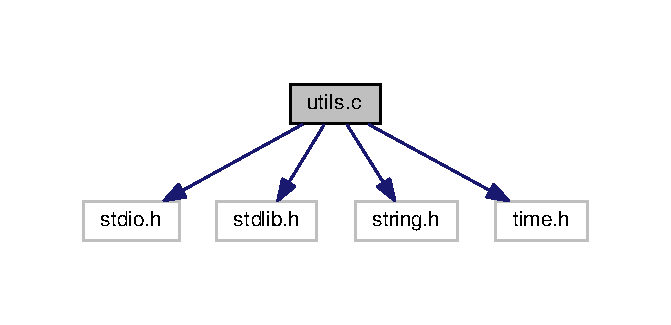
\includegraphics[width=322pt]{utils_8c__incl}
\end{center}
\end{figure}
\subsection*{Functions}
\begin{DoxyCompactItemize}
\item 
void \hyperlink{utils_8c_a9d7e8af417b6d543da691e9c0e2f6f9f}{clear\+Screen} ()
\item 
void \hyperlink{utils_8c_a821efd1de9257a6ac8bce69ecc1e5dfc}{init\+Matrix} (char tabuleiro\mbox{[}$\,$\mbox{]}\mbox{[}10\mbox{]})
\item 
void \hyperlink{utils_8c_a4898a09411ad503295bdbe640b05dd10}{print\+About} ()
\item 
void \hyperlink{utils_8c_aa4f7464685f4b851ed78ed3a99254372}{print\+Align} (int space, char $\ast$string)
\item 
void \hyperlink{utils_8c_a1ea6231221c4e03a66d89d0c38aa71cc}{print\+Battleship} ()
\item 
void \hyperlink{utils_8c_a087a2b7743093438ffebaedb708e3283}{print\+Menu1} ()
\item 
void \hyperlink{utils_8c_a4f2acb39a12d6c7570980ae92ec9befc}{print\+Menu2} ()
\item 
const char $\ast$ \hyperlink{utils_8c_afbbac206745f181d052cd054256405fb}{direction\+Message} (char direction)
\item 
const char $\ast$ \hyperlink{utils_8c_aa6fe75334720e315d3182069c55e3a68}{ship\+Name} (char ship)
\item 
const int \hyperlink{utils_8c_a35e15ea010d1f6dc8f27c9c574dec78e}{get\+Ship\+Size} (char ship)
\item 
int \hyperlink{utils_8c_aca751d22e44a1f046b2f3b14fecc84a6}{check\+Threshold} (int line, int col)
\item 
int \hyperlink{utils_8c_ad6cbd447e86b9eec5fe75e15370b3326}{check\+Coordenate} (char ship\+Type, char line, int col, char direction, char tabuleiro\mbox{[}$\,$\mbox{]}\mbox{[}10\mbox{]})
\item 
void \hyperlink{utils_8c_a362f75fd778db4d81e30c8e0f04495eb}{read\+Coordenate} (char $\ast$line, int $\ast$col)
\item 
void \hyperlink{utils_8c_a191c68084d72322fdfb77df4f0fefb4d}{check\+Shot} (char jogadas\mbox{[}$\,$\mbox{]}\mbox{[}10\mbox{]}, char tabuleiro\+Adversario\mbox{[}$\,$\mbox{]}\mbox{[}10\mbox{]}, char $\ast$nome\+Jogador, char $\ast$nome\+Adversario, int line, int col)
\item 
void \hyperlink{utils_8c_abec49bb0c079b81567289b409b10e4d9}{display\+Game\+Info} (char $\ast$nome\+Jogador1, char jogadas1\mbox{[}$\,$\mbox{]}\mbox{[}10\mbox{]}, char $\ast$nome\+Jogador2, char jogadas2\mbox{[}$\,$\mbox{]}\mbox{[}10\mbox{]})
\item 
void \hyperlink{utils_8c_ad3e46e8d515b2646486f391643333ed4}{display\+Game\+Player} (char $\ast$nome\+Jogador, char tabuleiro\mbox{[}$\,$\mbox{]}\mbox{[}10\mbox{]})
\item 
int \hyperlink{utils_8c_af4cf37339d3d98a2cbe99929874d9f02}{is\+End\+Game} (char jogadas\mbox{[}$\,$\mbox{]}\mbox{[}10\mbox{]})
\item 
void \hyperlink{utils_8c_a53aa17bcb66102859da0e09b78412911}{give\+Shot} (char jogadas\mbox{[}$\,$\mbox{]}\mbox{[}10\mbox{]}, char tabuleiro\+Adversario\mbox{[}$\,$\mbox{]}\mbox{[}10\mbox{]}, char $\ast$nome\+Jogador, char $\ast$nome\+Adversario)
\item 
void \hyperlink{utils_8c_a916e66ee495d0e5ac7d061cb882381f9}{give\+Random\+Shot} (char jogadas\mbox{[}$\,$\mbox{]}\mbox{[}10\mbox{]}, char tabuleiro\+Adversario\mbox{[}$\,$\mbox{]}\mbox{[}10\mbox{]}, char $\ast$nome\+Jogador, char $\ast$nome\+Adversario)
\item 
void \hyperlink{utils_8c_a92c29996f0bd795ae58310f30ba24466}{put\+Ship} (char ship\+Type, char line, int col, char direction, char tabuleiro\mbox{[}$\,$\mbox{]}\mbox{[}10\mbox{]})
\item 
void \hyperlink{utils_8c_a8dbfb8ff4e945c557e1baa84ca1c39fa}{put\+Ships} (char $\ast$nome\+Jogador, char tabuleiro\mbox{[}$\,$\mbox{]}\mbox{[}10\mbox{]})
\item 
void \hyperlink{utils_8c_ac2fd4847b2382dbddfea8eb84c01cdad}{put\+Ships\+C\+OM} (char tabuleiro\mbox{[}$\,$\mbox{]}\mbox{[}10\mbox{]})
\item 
void \hyperlink{utils_8c_a450dd23155e8a975d341985f105342c3}{print\+Resultados} (char $\ast$nome\+Jogador, char jogadas\mbox{[}$\,$\mbox{]}\mbox{[}10\mbox{]}, char tabuleiro\mbox{[}$\,$\mbox{]}\mbox{[}10\mbox{]})
\end{DoxyCompactItemize}


\subsection{Function Documentation}
\mbox{\Hypertarget{utils_8c_ad6cbd447e86b9eec5fe75e15370b3326}\label{utils_8c_ad6cbd447e86b9eec5fe75e15370b3326}} 
\index{utils.\+c@{utils.\+c}!check\+Coordenate@{check\+Coordenate}}
\index{check\+Coordenate@{check\+Coordenate}!utils.\+c@{utils.\+c}}
\subsubsection{\texorpdfstring{check\+Coordenate()}{checkCoordenate()}}
{\footnotesize\ttfamily int check\+Coordenate (\begin{DoxyParamCaption}\item[{char}]{ship\+Type,  }\item[{char}]{line,  }\item[{int}]{col,  }\item[{char}]{direction,  }\item[{char}]{tabuleiro\mbox{[}$\,$\mbox{]}\mbox{[}10\mbox{]} }\end{DoxyParamCaption})}

Verifica se a coordenada juntamente com a direção são válidas para inserção de uma embarcação no tabuleiro


\begin{DoxyParams}{Parameters}
{\em ship\+Type} & Tipo de embarcação \\
\hline
{\em line} & Linha da matriz \\
\hline
{\em col} & Coluna da matriz \\
\hline
{\em direction} & Direção do posicionamento da embarcação \\
\hline
{\em tabuleiro} & Tabuleiro do jogo \\
\hline
\end{DoxyParams}
\begin{DoxyReturn}{Returns}
1 se a coordenada é válida, 0 caso contrário 
\end{DoxyReturn}


Definition at line 168 of file utils.\+c.


\begin{DoxyCode}
168                                                                                             \{
169     \textcolor{keywordtype}{int} intLine = (int)line-65;
170     \textcolor{comment}{/* Verifico:}
171 \textcolor{comment}{     * - se é uma coordenada dentro da matriz}
172 \textcolor{comment}{     * - se a letra informada para a direção é válida}
173 \textcolor{comment}{     * - se a direção e a coordenada ficam dentro da matriz}
174 \textcolor{comment}{    */}
175     \textcolor{keywordflow}{if}(!\hyperlink{utils_8c_aca751d22e44a1f046b2f3b14fecc84a6}{checkThreshold}(intLine, col) 
176         || !(direction == \textcolor{charliteral}{'W'} || direction == \textcolor{charliteral}{'S'} || direction == \textcolor{charliteral}{'A'} || direction == \textcolor{charliteral}{'D'})
177         || (direction == \textcolor{charliteral}{'W'} && (intLine - \hyperlink{utils_8c_a35e15ea010d1f6dc8f27c9c574dec78e}{getShipSize}(shipType) < 0))
178         || (direction == \textcolor{charliteral}{'S'} && (intLine + \hyperlink{utils_8c_a35e15ea010d1f6dc8f27c9c574dec78e}{getShipSize}(shipType) > 10))
179         || (direction == \textcolor{charliteral}{'A'} && (col - \hyperlink{utils_8c_a35e15ea010d1f6dc8f27c9c574dec78e}{getShipSize}(shipType) < 0))
180         || (direction == \textcolor{charliteral}{'D'} && (col + \hyperlink{utils_8c_a35e15ea010d1f6dc8f27c9c574dec78e}{getShipSize}(shipType) > 10)))\{
181         \textcolor{keywordflow}{return} 0;
182     \}
183 
184     \textcolor{comment}{// Verifico se as posições em que a embarcação será colocada estão livres}
185     \textcolor{keywordflow}{switch}(direction)\{
186         \textcolor{keywordflow}{case} \textcolor{charliteral}{'W'}:
187             \textcolor{comment}{//"Para Cima"}
188             \textcolor{keywordflow}{for}(\textcolor{keywordtype}{int} i = intLine; i > (intLine - \hyperlink{utils_8c_a35e15ea010d1f6dc8f27c9c574dec78e}{getShipSize}(shipType)); i--)\{
189                 \textcolor{keywordflow}{if}(tabuleiro[i][col] != \textcolor{charliteral}{'.'})\{
190                     \textcolor{keywordflow}{return} 0;
191                 \}
192             \}
193             \textcolor{keywordflow}{break};
194         \textcolor{keywordflow}{case} \textcolor{charliteral}{'S'}:
195             \textcolor{comment}{//"Para Baixo"}
196             \textcolor{keywordflow}{for}(\textcolor{keywordtype}{int} i = intLine; i < (intLine + \hyperlink{utils_8c_a35e15ea010d1f6dc8f27c9c574dec78e}{getShipSize}(shipType)); i++)\{
197                 \textcolor{keywordflow}{if}(tabuleiro[i][col] != \textcolor{charliteral}{'.'})\{
198                     \textcolor{keywordflow}{return} 0;
199                 \}
200             \}
201             \textcolor{keywordflow}{break};
202         \textcolor{keywordflow}{case} \textcolor{charliteral}{'D'}:
203             \textcolor{comment}{//"Para Direita"}
204             \textcolor{keywordflow}{for}(\textcolor{keywordtype}{int} i = col; i < (col + \hyperlink{utils_8c_a35e15ea010d1f6dc8f27c9c574dec78e}{getShipSize}(shipType)); i++)\{
205                 \textcolor{keywordflow}{if}(tabuleiro[intLine][i] != \textcolor{charliteral}{'.'})\{
206                     \textcolor{keywordflow}{return} 0;
207                 \}
208             \}
209             \textcolor{keywordflow}{break};
210         \textcolor{keywordflow}{case} \textcolor{charliteral}{'A'}:
211             \textcolor{comment}{//"Para Esquerda"}
212             \textcolor{keywordflow}{for}(\textcolor{keywordtype}{int} i = col; i > (col - \hyperlink{utils_8c_a35e15ea010d1f6dc8f27c9c574dec78e}{getShipSize}(shipType)); i--)\{
213                 \textcolor{keywordflow}{if}(tabuleiro[intLine][i] != \textcolor{charliteral}{'.'})\{
214                     \textcolor{keywordflow}{return} 0;
215                 \}
216             \}
217             \textcolor{keywordflow}{break};
218     \}
219 
220     \textcolor{keywordflow}{return} 1;
221 \}
\end{DoxyCode}
\mbox{\Hypertarget{utils_8c_a191c68084d72322fdfb77df4f0fefb4d}\label{utils_8c_a191c68084d72322fdfb77df4f0fefb4d}} 
\index{utils.\+c@{utils.\+c}!check\+Shot@{check\+Shot}}
\index{check\+Shot@{check\+Shot}!utils.\+c@{utils.\+c}}
\subsubsection{\texorpdfstring{check\+Shot()}{checkShot()}}
{\footnotesize\ttfamily void check\+Shot (\begin{DoxyParamCaption}\item[{char}]{jogadas\mbox{[}$\,$\mbox{]}\mbox{[}10\mbox{]},  }\item[{char}]{tabuleiro\+Adversario\mbox{[}$\,$\mbox{]}\mbox{[}10\mbox{]},  }\item[{char $\ast$}]{nome\+Jogador,  }\item[{char $\ast$}]{nome\+Adversario,  }\item[{int}]{line,  }\item[{int}]{col }\end{DoxyParamCaption})}

Verifica o resultado de uma jogada (disparo) da batalha naval


\begin{DoxyParams}{Parameters}
{\em jogadas} & Jogadas realizadas pelo jogador até o momento. \\
\hline
{\em tabuleiro\+Adversario} & Tabuleiro do adversário \\
\hline
{\em nome\+Jogador} & Nome do jogador \\
\hline
{\em nome\+Adversario} & Nome do adversário \\
\hline
\end{DoxyParams}


Definition at line 254 of file utils.\+c.


\begin{DoxyCode}
254                                                                                                            
                         \{
255     \hyperlink{utils_8c_a9d7e8af417b6d543da691e9c0e2f6f9f}{clearScreen}();
256     \hyperlink{utils_8c_a1ea6231221c4e03a66d89d0c38aa71cc}{printBattleship}();
257     printf(\textcolor{stringliteral}{"\(\backslash\)n\(\backslash\)n"});
258 
259     printf(\textcolor{stringliteral}{"Resultado do disparo realizado por: %s\(\backslash\)n\(\backslash\)n"}, nomeJogador);
260 
261     printf(\textcolor{stringliteral}{"*****************************************************************\(\backslash\)n"});
262     \textcolor{comment}{// Verifico onde o disparo acertou e atribuo o indicador}
263     \textcolor{keywordflow}{if}(tabuleiroAdversario[line][col] == \textcolor{charliteral}{'.'})\{
264         jogadas[line][col] = \textcolor{charliteral}{'O'};
265         printf(\textcolor{stringliteral}{"* Água! \(\backslash\)n"});
266     \}\textcolor{keywordflow}{else}\{
267         printf(\textcolor{stringliteral}{"* Fogo! \(\backslash\)n"});
268         jogadas[line][col] = \textcolor{charliteral}{'X'};
269 
270         \textcolor{keywordtype}{char} shipType = tabuleiroAdversario[line][col]; \textcolor{comment}{// Guardo o tipo de embarcação atingida}
271         \textcolor{keywordtype}{int} contHits = 0; \textcolor{comment}{// Quantas vezes essa embarcação foi atingida}
272 
273         \textcolor{comment}{// Verifico se minha embarcação afundou}
274         \textcolor{keywordflow}{for}(\textcolor{keywordtype}{int} i = 0; i < 10; i ++)\{
275             \textcolor{keywordflow}{for}(\textcolor{keywordtype}{int} j = 0; j < 10; j++)\{
276                 \textcolor{comment}{// Se há um disparo para minha embarcação, acumulo o número de vezes que ela foi acertada}
277                 \textcolor{keywordflow}{if}(jogadas[i][j] == \textcolor{charliteral}{'X'} && tabuleiroAdversario[i][j] == shipType)\{
278                     contHits++;
279                 \}
280             \}
281         \}
282 
283         \textcolor{comment}{// Se acertei o número de vezes igual ao tamanho dela, significa que afundei a embarcação}
284         \textcolor{keywordflow}{if}(contHits == \hyperlink{utils_8c_a35e15ea010d1f6dc8f27c9c574dec78e}{getShipSize}(shipType))\{
285             printf(\textcolor{stringliteral}{"* %s: Afundou %s %s!\(\backslash\)n"}, nomeAdversario, shipType == \textcolor{charliteral}{'N'} ? \textcolor{stringliteral}{"minha"} : \textcolor{stringliteral}{"meu"}, 
      \hyperlink{utils_8c_aa6fe75334720e315d3182069c55e3a68}{shipName}(shipType));
286 
287             \textcolor{comment}{// Mostro no tabuleiro minha embarcação}
288             \textcolor{keywordflow}{for}(\textcolor{keywordtype}{int} i = 0; i < 10; i ++)\{
289                 \textcolor{keywordflow}{for}(\textcolor{keywordtype}{int} j = 0; j < 10; j++)\{
290                     \textcolor{comment}{// Procuro as posições da embarcação afundada e coloco a sigla dela para ser mostrada}
291                     \textcolor{keywordflow}{if}(tabuleiroAdversario[i][j] == shipType)\{
292                         jogadas[i][j] = shipType;
293                     \}
294                 \}
295             \}
296         \}
297     \}
298     printf(\textcolor{stringliteral}{"*****************************************************************\(\backslash\)n"});
299     printf(\textcolor{stringliteral}{"\(\backslash\)n\(\backslash\)n\(\backslash\)n"});
300 \}
\end{DoxyCode}
\mbox{\Hypertarget{utils_8c_aca751d22e44a1f046b2f3b14fecc84a6}\label{utils_8c_aca751d22e44a1f046b2f3b14fecc84a6}} 
\index{utils.\+c@{utils.\+c}!check\+Threshold@{check\+Threshold}}
\index{check\+Threshold@{check\+Threshold}!utils.\+c@{utils.\+c}}
\subsubsection{\texorpdfstring{check\+Threshold()}{checkThreshold()}}
{\footnotesize\ttfamily int check\+Threshold (\begin{DoxyParamCaption}\item[{int}]{line,  }\item[{int}]{col }\end{DoxyParamCaption})}

Verifica se a coordenada é válidas para inserção de uma embarcação no tabuleiro


\begin{DoxyParams}{Parameters}
{\em line} & Linha da matriz \\
\hline
{\em col} & Coluna da matriz \\
\hline
\end{DoxyParams}
\begin{DoxyReturn}{Returns}
1 se a coordenada é válida, 0 caso contrário 
\end{DoxyReturn}


Definition at line 154 of file utils.\+c.


\begin{DoxyCode}
154                                      \{
155     \textcolor{keywordflow}{return} !(line < 0 || col < 0 || line > 10 || col > 10);
156 \}
\end{DoxyCode}
\mbox{\Hypertarget{utils_8c_a9d7e8af417b6d543da691e9c0e2f6f9f}\label{utils_8c_a9d7e8af417b6d543da691e9c0e2f6f9f}} 
\index{utils.\+c@{utils.\+c}!clear\+Screen@{clear\+Screen}}
\index{clear\+Screen@{clear\+Screen}!utils.\+c@{utils.\+c}}
\subsubsection{\texorpdfstring{clear\+Screen()}{clearScreen()}}
{\footnotesize\ttfamily void clear\+Screen (\begin{DoxyParamCaption}{ }\end{DoxyParamCaption})}

Limpa a tela do console 

Definition at line 18 of file utils.\+c.


\begin{DoxyCode}
18                   \{
19   system(\textcolor{stringliteral}{"@cls||clear"});
20 \}
\end{DoxyCode}
\mbox{\Hypertarget{utils_8c_afbbac206745f181d052cd054256405fb}\label{utils_8c_afbbac206745f181d052cd054256405fb}} 
\index{utils.\+c@{utils.\+c}!direction\+Message@{direction\+Message}}
\index{direction\+Message@{direction\+Message}!utils.\+c@{utils.\+c}}
\subsubsection{\texorpdfstring{direction\+Message()}{directionMessage()}}
{\footnotesize\ttfamily const char$\ast$ direction\+Message (\begin{DoxyParamCaption}\item[{char}]{direction }\end{DoxyParamCaption})}

Retorna a mensagem correspondende à cada direção 

Definition at line 98 of file utils.\+c.


\begin{DoxyCode}
98                                              \{
99     \textcolor{keywordflow}{switch}(direction)\{
100         \textcolor{keywordflow}{case} \textcolor{charliteral}{'W'}:
101             \textcolor{keywordflow}{return} \textcolor{stringliteral}{"Para Cima"};
102         \textcolor{keywordflow}{case} \textcolor{charliteral}{'S'}:
103             \textcolor{keywordflow}{return} \textcolor{stringliteral}{"Para Baixo"};
104         \textcolor{keywordflow}{case} \textcolor{charliteral}{'D'}:
105             \textcolor{keywordflow}{return} \textcolor{stringliteral}{"Para Direita"};
106         \textcolor{keywordflow}{case} \textcolor{charliteral}{'A'}:
107             \textcolor{keywordflow}{return} \textcolor{stringliteral}{"Para Esquerda"};
108     \} 
109 \}
\end{DoxyCode}
\mbox{\Hypertarget{utils_8c_abec49bb0c079b81567289b409b10e4d9}\label{utils_8c_abec49bb0c079b81567289b409b10e4d9}} 
\index{utils.\+c@{utils.\+c}!display\+Game\+Info@{display\+Game\+Info}}
\index{display\+Game\+Info@{display\+Game\+Info}!utils.\+c@{utils.\+c}}
\subsubsection{\texorpdfstring{display\+Game\+Info()}{displayGameInfo()}}
{\footnotesize\ttfamily void display\+Game\+Info (\begin{DoxyParamCaption}\item[{char $\ast$}]{nome\+Jogador1,  }\item[{char}]{jogadas1\mbox{[}$\,$\mbox{]}\mbox{[}10\mbox{]},  }\item[{char $\ast$}]{nome\+Jogador2,  }\item[{char}]{jogadas2\mbox{[}$\,$\mbox{]}\mbox{[}10\mbox{]} }\end{DoxyParamCaption})}

Mostra as informações dos tabuleiros lado a lado de dois jogadores com os seus respectivos nomes. Exemplo\+: Player $\vert$ Computer 0 1 2 3 4 5 6 7 8 9 $\vert$ 0 1 2 3 4 5 6 7 8 9 A $\vert$\+P$\vert$ $\vert$ $\vert$ $\vert$ $\vert$ $\vert$ $\vert$ $\vert$ $\vert$ $\vert$ $\vert$ A $\vert$ $\vert$ $\vert$ $\vert$ $\vert$ $\vert$ $\vert$ $\vert$ $\vert$ $\vert$ $\vert$ B $\vert$\+P$\vert$ $\vert$ $\vert$ $\vert$ $\vert$ $\vert$ $\vert$ $\vert$ $\vert$ $\vert$ $\vert$ B $\vert$ $\vert$ $\vert$ $\vert$ $\vert$ $\vert$ $\vert$ $\vert$ $\vert$ $\vert$ $\vert$ C $\vert$\+P$\vert$ $\vert$ $\vert$ $\vert$ $\vert$ $\vert$ $\vert$ $\vert$ $\vert$ $\vert$ $\vert$ C $\vert$ $\vert$ $\vert$ $\vert$ $\vert$ $\vert$ $\vert$\+O$\vert$ $\vert$ $\vert$ $\vert$ D $\vert$\+P$\vert$ $\vert$ $\vert$ $\vert$ $\vert$ $\vert$ $\vert$ $\vert$ $\vert$ $\vert$ $\vert$ D $\vert$ $\vert$ $\vert$x$\vert$ $\vert$ $\vert$ $\vert$ $\vert$ $\vert$ $\vert$ $\vert$ E $\vert$\+P$\vert$ $\vert$ $\vert$ $\vert$ $\vert$ $\vert$ $\vert$ $\vert$ $\vert$ $\vert$ $\vert$ E $\vert$ $\vert$ $\vert$ $\vert$ $\vert$ $\vert$ $\vert$ $\vert$ $\vert$ $\vert$ $\vert$ F $\vert$ $\vert$ $\vert$ $\vert$ $\vert$ $\vert$ $\vert$ $\vert$ $\vert$ $\vert$ $\vert$ $\vert$ F $\vert$ $\vert$ $\vert$ $\vert$ $\vert$\+O$\vert$ $\vert$ $\vert$ $\vert$ $\vert$ $\vert$ G $\vert$ $\vert$ $\vert$ $\vert$ $\vert$ $\vert$ $\vert$ $\vert$ $\vert$ $\vert$ $\vert$ $\vert$ G $\vert$ $\vert$ $\vert$ $\vert$ $\vert$ $\vert$ $\vert$ $\vert$ $\vert$ $\vert$ $\vert$ H $\vert$ $\vert$ $\vert$ $\vert$ $\vert$ $\vert$ $\vert$ $\vert$ $\vert$ $\vert$ $\vert$ $\vert$ H $\vert$ $\vert$\+O$\vert$ $\vert$ $\vert$ $\vert$ $\vert$\+O$\vert$ $\vert$ $\vert$ $\vert$ I $\vert$ $\vert$ $\vert$ $\vert$ $\vert$ $\vert$ $\vert$ $\vert$ $\vert$ $\vert$ $\vert$ $\vert$ I $\vert$ $\vert$ $\vert$ $\vert$ $\vert$ $\vert$ $\vert$ $\vert$ $\vert$ $\vert$ $\vert$ J $\vert$ $\vert$ $\vert$ $\vert$ $\vert$ $\vert$ $\vert$ $\vert$ $\vert$ $\vert$ $\vert$ $\vert$ J $\vert$ $\vert$ $\vert$ $\vert$ $\vert$ $\vert$ $\vert$ $\vert$ $\vert$ $\vert$ $\vert$


\begin{DoxyParams}{Parameters}
{\em nome\+Jogador1} & Nome do jogador 1 \\
\hline
{\em jogadas1} & Tabuleiro de jogadas do jogador 1 \\
\hline
{\em nome\+Jogador2} & Nome do jogador 2 \\
\hline
{\em jogadas2} & Tabuleiro de jogadas do jogador 2 \\
\hline
\end{DoxyParams}


Definition at line 323 of file utils.\+c.


\begin{DoxyCode}
323                                                                                                       \{
324     \textcolor{keywordtype}{char} separador[] = \textcolor{stringliteral}{"     |   "};
325 
326     \textcolor{comment}{// Imprimo o cabeçalho}
327     \hyperlink{utils_8c_aa4f7464685f4b851ed78ed3a99254372}{printAlign}(41, nomeJogador1);
328     printf(\textcolor{stringliteral}{"%s"}, separador);
329     \hyperlink{utils_8c_aa4f7464685f4b851ed78ed3a99254372}{printAlign}(44, nomeJogador2);
330     printf(\textcolor{stringliteral}{"\(\backslash\)n"});
331 
332     \textcolor{keywordflow}{for}(\textcolor{keywordtype}{int} cont = 0; cont < 2; cont++)\{
333         printf(\textcolor{stringliteral}{" "});
334         \textcolor{keywordflow}{for} (\textcolor{keywordtype}{int} i = 0; i < 10; i++) \{
335             printf(\textcolor{stringliteral}{"   %i"}, i);
336         \}
337         \textcolor{keywordflow}{if}(!cont)\{
338             printf(\textcolor{stringliteral}{"%s"}, separador);
339         \}
340     \}
341     printf(\textcolor{stringliteral}{"\(\backslash\)n"});
342     
343     \textcolor{comment}{// Imprimo as linhas}
344     \textcolor{keywordflow}{for} (\textcolor{keywordtype}{int} i = 0; i < 10; i++) \{
345         \textcolor{comment}{// Imprime a letra}
346         printf(\textcolor{stringliteral}{"%c | "}, 65+i);
347 
348         \textcolor{comment}{// Imprime os valores do player1}
349         \textcolor{keywordflow}{for} (\textcolor{keywordtype}{int} j = 0; j < 10; j++) \{
350             printf(\textcolor{stringliteral}{"%c | "}, jogadas1[i][j]);
351         \}
352 
353         \textcolor{comment}{// Imprime a letra}
354         printf(\textcolor{stringliteral}{"  |   %c | "}, 65+i);
355         \textcolor{comment}{// Imprime os valores do player 2}
356         \textcolor{keywordflow}{for} (\textcolor{keywordtype}{int} j = 0; j < 10; j++) \{
357             printf(\textcolor{stringliteral}{"%c | "}, jogadas2[i][j]);
358         \}
359         printf(\textcolor{stringliteral}{"\(\backslash\)n"});
360     \}
361 \}
\end{DoxyCode}
\mbox{\Hypertarget{utils_8c_ad3e46e8d515b2646486f391643333ed4}\label{utils_8c_ad3e46e8d515b2646486f391643333ed4}} 
\index{utils.\+c@{utils.\+c}!display\+Game\+Player@{display\+Game\+Player}}
\index{display\+Game\+Player@{display\+Game\+Player}!utils.\+c@{utils.\+c}}
\subsubsection{\texorpdfstring{display\+Game\+Player()}{displayGamePlayer()}}
{\footnotesize\ttfamily void display\+Game\+Player (\begin{DoxyParamCaption}\item[{char $\ast$}]{nome\+Jogador,  }\item[{char}]{tabuleiro\mbox{[}$\,$\mbox{]}\mbox{[}10\mbox{]} }\end{DoxyParamCaption})}

Mostra as informações do tabuleiro do jogador com os seu respectivo nome. Exemplo\+: Player 0 1 2 3 4 5 6 7 8 9 A $\vert$\+P$\vert$ $\vert$ $\vert$ $\vert$ $\vert$ $\vert$ $\vert$ $\vert$ $\vert$ $\vert$ B $\vert$\+P$\vert$ $\vert$ $\vert$ $\vert$ $\vert$ $\vert$ $\vert$ $\vert$ $\vert$ $\vert$ C $\vert$\+P$\vert$ $\vert$ $\vert$ $\vert$ $\vert$ $\vert$ $\vert$ $\vert$ $\vert$ $\vert$ D $\vert$\+P$\vert$ $\vert$ $\vert$ $\vert$ $\vert$ $\vert$ $\vert$ $\vert$ $\vert$ $\vert$ E $\vert$\+P$\vert$ $\vert$ $\vert$ $\vert$ $\vert$ $\vert$ $\vert$ $\vert$ $\vert$ $\vert$ F $\vert$ $\vert$ $\vert$ $\vert$ $\vert$ $\vert$ $\vert$ $\vert$ $\vert$ $\vert$ $\vert$ G $\vert$ $\vert$ $\vert$ $\vert$ $\vert$\+N$\vert$\+N$\vert$\+N$\vert$ $\vert$ $\vert$ $\vert$ H $\vert$ $\vert$ $\vert$ $\vert$ $\vert$ $\vert$ $\vert$ $\vert$ $\vert$ $\vert$ $\vert$ I $\vert$ $\vert$ $\vert$ $\vert$ $\vert$ $\vert$ $\vert$ $\vert$ $\vert$ $\vert$ $\vert$ J $\vert$ $\vert$ $\vert$ $\vert$ $\vert$ $\vert$ $\vert$ $\vert$ $\vert$ $\vert$ $\vert$


\begin{DoxyParams}{Parameters}
{\em nome\+Jogador} & Nome do jogador \\
\hline
{\em tabuleiro} & Tabuleiro do jogador \\
\hline
\end{DoxyParams}


Definition at line 382 of file utils.\+c.


\begin{DoxyCode}
382                                                                \{
383     \textcolor{keywordtype}{char} separador[] = \textcolor{stringliteral}{"     |   "};
384 
385     \textcolor{comment}{// Imprimo o cabeçalho}
386     \hyperlink{utils_8c_aa4f7464685f4b851ed78ed3a99254372}{printAlign}(41, nomeJogador);
387     printf(\textcolor{stringliteral}{"\(\backslash\)n"});
388     
389     printf(\textcolor{stringliteral}{" "});
390     \textcolor{keywordflow}{for} (\textcolor{keywordtype}{int} i = 0; i < 10; i++) \{
391         printf(\textcolor{stringliteral}{"   %i"}, i);
392     \}
393     printf(\textcolor{stringliteral}{"\(\backslash\)n"});
394     
395     \textcolor{comment}{// Imprimo as linhas}
396     \textcolor{keywordflow}{for} (\textcolor{keywordtype}{int} i = 0; i < 10; i++) \{
397         \textcolor{comment}{// Imprime a letra}
398         printf(\textcolor{stringliteral}{"%c | "}, 65+i);
399 
400         \textcolor{comment}{// Imprime os valores do jogador}
401         \textcolor{keywordflow}{for} (\textcolor{keywordtype}{int} j = 0; j < 10; j++) \{
402             printf(\textcolor{stringliteral}{"%c | "}, tabuleiro[i][j]);
403         \}
404         printf(\textcolor{stringliteral}{"\(\backslash\)n"});
405     \}
406 \}
\end{DoxyCode}
\mbox{\Hypertarget{utils_8c_a35e15ea010d1f6dc8f27c9c574dec78e}\label{utils_8c_a35e15ea010d1f6dc8f27c9c574dec78e}} 
\index{utils.\+c@{utils.\+c}!get\+Ship\+Size@{get\+Ship\+Size}}
\index{get\+Ship\+Size@{get\+Ship\+Size}!utils.\+c@{utils.\+c}}
\subsubsection{\texorpdfstring{get\+Ship\+Size()}{getShipSize()}}
{\footnotesize\ttfamily const int get\+Ship\+Size (\begin{DoxyParamCaption}\item[{char}]{ship }\end{DoxyParamCaption})}

Retorna o tamanho da embarcação de acordo com a sigla 

Definition at line 132 of file utils.\+c.


\begin{DoxyCode}
132                                 \{
133     \textcolor{keywordflow}{switch}(ship)\{
134         \textcolor{keywordflow}{case} \textcolor{charliteral}{'P'}:
135             \textcolor{keywordflow}{return} 5;
136         \textcolor{keywordflow}{case} \textcolor{charliteral}{'N'}:
137             \textcolor{keywordflow}{return} 4;
138         \textcolor{keywordflow}{case} \textcolor{charliteral}{'C'}:
139             \textcolor{keywordflow}{return} 3;
140         \textcolor{keywordflow}{case} \textcolor{charliteral}{'S'}:
141             \textcolor{keywordflow}{return} 3;
142         \textcolor{keywordflow}{case} \textcolor{charliteral}{'D'}:
143             \textcolor{keywordflow}{return} 2;
144     \}
145 \}
\end{DoxyCode}
\mbox{\Hypertarget{utils_8c_a916e66ee495d0e5ac7d061cb882381f9}\label{utils_8c_a916e66ee495d0e5ac7d061cb882381f9}} 
\index{utils.\+c@{utils.\+c}!give\+Random\+Shot@{give\+Random\+Shot}}
\index{give\+Random\+Shot@{give\+Random\+Shot}!utils.\+c@{utils.\+c}}
\subsubsection{\texorpdfstring{give\+Random\+Shot()}{giveRandomShot()}}
{\footnotesize\ttfamily void give\+Random\+Shot (\begin{DoxyParamCaption}\item[{char}]{jogadas\mbox{[}$\,$\mbox{]}\mbox{[}10\mbox{]},  }\item[{char}]{tabuleiro\+Adversario\mbox{[}$\,$\mbox{]}\mbox{[}10\mbox{]},  }\item[{char $\ast$}]{nome\+Jogador,  }\item[{char $\ast$}]{nome\+Adversario }\end{DoxyParamCaption})}

A máquina realiza uma jogada (disparo) da batalha naval


\begin{DoxyParams}{Parameters}
{\em jogadas} & Jogadas realizadas pelo jogador até o momento. \\
\hline
{\em tabuleiro\+Adversario} & Tabuleiro do adversário \\
\hline
{\em nome\+Jogador} & Nome do jogador \\
\hline
{\em nome\+Adversario} & Nome do adversário \\
\hline
\end{DoxyParams}


Definition at line 492 of file utils.\+c.


\begin{DoxyCode}
492                                                                                                            
           \{
493     \textcolor{keywordtype}{int} col, line;
494     
495     \textcolor{keywordflow}{do}\{
496         srand(time(NULL));
497         line = rand() % 10;
498         col = rand() % 10;
499         
500         \textcolor{keywordflow}{if}(jogadas[line][col] == \textcolor{charliteral}{'.'})\{
501             \textcolor{keywordflow}{break};
502         \}
503     \}\textcolor{keywordflow}{while}(1);
504 
505     \hyperlink{utils_8c_a191c68084d72322fdfb77df4f0fefb4d}{checkShot}(jogadas, tabuleiroAdversario, nomeJogador, nomeAdversario, line, col);
506 \}
\end{DoxyCode}
\mbox{\Hypertarget{utils_8c_a53aa17bcb66102859da0e09b78412911}\label{utils_8c_a53aa17bcb66102859da0e09b78412911}} 
\index{utils.\+c@{utils.\+c}!give\+Shot@{give\+Shot}}
\index{give\+Shot@{give\+Shot}!utils.\+c@{utils.\+c}}
\subsubsection{\texorpdfstring{give\+Shot()}{giveShot()}}
{\footnotesize\ttfamily void give\+Shot (\begin{DoxyParamCaption}\item[{char}]{jogadas\mbox{[}$\,$\mbox{]}\mbox{[}10\mbox{]},  }\item[{char}]{tabuleiro\+Adversario\mbox{[}$\,$\mbox{]}\mbox{[}10\mbox{]},  }\item[{char $\ast$}]{nome\+Jogador,  }\item[{char $\ast$}]{nome\+Adversario }\end{DoxyParamCaption})}

Realiza uma jogada (disparo) da batalha naval por um jogador


\begin{DoxyParams}{Parameters}
{\em jogadas} & Jogadas realizadas pelo jogador até o momento. \\
\hline
{\em tabuleiro\+Adversario} & Tabuleiro do adversário \\
\hline
{\em nome\+Jogador} & Nome do jogador \\
\hline
{\em nome\+Adversario} & Nome do adversário \\
\hline
\end{DoxyParams}


Definition at line 464 of file utils.\+c.


\begin{DoxyCode}
464                                                                                                           \{
465     \textcolor{keywordtype}{int} col, intLine;
466     \textcolor{keywordtype}{char} line;
467 
468     \textcolor{comment}{// O programa solicita um disparo válido}
469     \textcolor{keywordflow}{do}\{
470         \hyperlink{utils_8c_a362f75fd778db4d81e30c8e0f04495eb}{readCoordenate}(&line, &col);
471 
472         intLine = (int)line-65;
473 
474         \textcolor{keywordflow}{if}(jogadas[intLine][col] == \textcolor{charliteral}{'.'})\{
475             \textcolor{keywordflow}{break};
476         \}\textcolor{keywordflow}{else}\{
477             printf(\textcolor{stringliteral}{"Essa coordenada já foi informada anteriormente. Tente novamente.\(\backslash\)n"});
478         \}       
479     \}\textcolor{keywordflow}{while}(1);
480 
481     \hyperlink{utils_8c_a191c68084d72322fdfb77df4f0fefb4d}{checkShot}(jogadas, tabuleiroAdversario, nomeJogador, nomeAdversario, intLine, col);
482 \}
\end{DoxyCode}
\mbox{\Hypertarget{utils_8c_a821efd1de9257a6ac8bce69ecc1e5dfc}\label{utils_8c_a821efd1de9257a6ac8bce69ecc1e5dfc}} 
\index{utils.\+c@{utils.\+c}!init\+Matrix@{init\+Matrix}}
\index{init\+Matrix@{init\+Matrix}!utils.\+c@{utils.\+c}}
\subsubsection{\texorpdfstring{init\+Matrix()}{initMatrix()}}
{\footnotesize\ttfamily void init\+Matrix (\begin{DoxyParamCaption}\item[{char}]{tabuleiro\mbox{[}$\,$\mbox{]}\mbox{[}10\mbox{]} }\end{DoxyParamCaption})}

Inicializo cada posição do tabuleiro do jogador com \textquotesingle{}.\textquotesingle{}


\begin{DoxyParams}{Parameters}
{\em tabuleiro} & Tabuleiro do jogador \\
\hline
\end{DoxyParams}


Definition at line 27 of file utils.\+c.


\begin{DoxyCode}
27                                      \{
28     \textcolor{keywordflow}{for} (\textcolor{keywordtype}{int} i = 0; i < 10; i++) \{      
29       \textcolor{keywordflow}{for} (\textcolor{keywordtype}{int} j = 0; j < 10; j++) \{
30         tabuleiro[i][j] = \textcolor{charliteral}{'.'};
31       \}      
32     \}
33 \}
\end{DoxyCode}
\mbox{\Hypertarget{utils_8c_af4cf37339d3d98a2cbe99929874d9f02}\label{utils_8c_af4cf37339d3d98a2cbe99929874d9f02}} 
\index{utils.\+c@{utils.\+c}!is\+End\+Game@{is\+End\+Game}}
\index{is\+End\+Game@{is\+End\+Game}!utils.\+c@{utils.\+c}}
\subsubsection{\texorpdfstring{is\+End\+Game()}{isEndGame()}}
{\footnotesize\ttfamily int is\+End\+Game (\begin{DoxyParamCaption}\item[{char}]{jogadas\mbox{[}$\,$\mbox{]}\mbox{[}10\mbox{]} }\end{DoxyParamCaption})}

Verifica se o jogo já acabou


\begin{DoxyParams}{Parameters}
{\em jogadas} & Tabuleiro de jogadas de algum jogador \\
\hline
\end{DoxyParams}
\begin{DoxyReturn}{Returns}
Retorna 1 se todas as embarcações foram afundadas, 0 caso contrário 
\end{DoxyReturn}


Definition at line 414 of file utils.\+c.


\begin{DoxyCode}
414                                  \{
415     \textcolor{keywordtype}{int} embarcacoesAfundadas = 0;
416 
417     \textcolor{comment}{// Verifico se todas as embarcações foram afundadas}
418     \textcolor{keywordflow}{for}(\textcolor{keywordtype}{int} i = 0; i < 5; i++)\{
419 
420         \textcolor{keywordtype}{char} shipType;
421 
422         \textcolor{keywordflow}{switch}(i)\{
423             \textcolor{keywordflow}{case} 0:
424                 shipType = \textcolor{charliteral}{'P'};
425                 \textcolor{keywordflow}{break};
426             \textcolor{keywordflow}{case} 1:
427                 shipType = \textcolor{charliteral}{'N'};
428                 \textcolor{keywordflow}{break};
429             \textcolor{keywordflow}{case} 2:
430                 shipType = \textcolor{charliteral}{'C'};
431                 \textcolor{keywordflow}{break};
432             \textcolor{keywordflow}{case} 3:
433                 shipType = \textcolor{charliteral}{'S'};
434                 \textcolor{keywordflow}{break};
435             \textcolor{keywordflow}{case} 4:
436                 shipType = \textcolor{charliteral}{'D'};
437                 \textcolor{keywordflow}{break};
438         \}
439 
440         \textcolor{comment}{// Se o tabuleiro contém a letra da embarcação significa que essa embarcação foi afundada}
441         \textcolor{keywordflow}{for}(\textcolor{keywordtype}{int} i = 0; i < 10; i++)\{
442             \textcolor{keywordflow}{for}(\textcolor{keywordtype}{int} j = 0; j < 10; j++)\{
443                 \textcolor{keywordflow}{if}(jogadas[i][j] == shipType)\{
444                     embarcacoesAfundadas++;
445                     i = j = 10;
446                     \textcolor{keywordflow}{break};
447                 \}
448             \}
449         \}
450     \}
451 
452     
453     \textcolor{keywordflow}{return} embarcacoesAfundadas == 5 ? 1 : 0;
454 \}
\end{DoxyCode}
\mbox{\Hypertarget{utils_8c_a4898a09411ad503295bdbe640b05dd10}\label{utils_8c_a4898a09411ad503295bdbe640b05dd10}} 
\index{utils.\+c@{utils.\+c}!print\+About@{print\+About}}
\index{print\+About@{print\+About}!utils.\+c@{utils.\+c}}
\subsubsection{\texorpdfstring{print\+About()}{printAbout()}}
{\footnotesize\ttfamily void print\+About (\begin{DoxyParamCaption}{ }\end{DoxyParamCaption})}

Mostra as informações sobre o jogo 

Definition at line 38 of file utils.\+c.


\begin{DoxyCode}
38                  \{
39     printf(\textcolor{stringliteral}{"**************************************************************\(\backslash\)n"});
40     printf(\textcolor{stringliteral}{"*Bem-vindo ao jogo de batalha naval! - Exemplo trabalho UFPR *\(\backslash\)n"});
41     printf(\textcolor{stringliteral}{"**************************************************************\(\backslash\)n"});
42     printf(\textcolor{stringliteral}{"\(\backslash\)n\(\backslash\)n\(\backslash\)n"});
43     printf(\textcolor{stringliteral}{"Esse exemplo foi desenvolvido por Jackson Antonio do Prado Lima.\(\backslash\)n\(\backslash\)n\(\backslash\)n"});
44 \}
\end{DoxyCode}
\mbox{\Hypertarget{utils_8c_aa4f7464685f4b851ed78ed3a99254372}\label{utils_8c_aa4f7464685f4b851ed78ed3a99254372}} 
\index{utils.\+c@{utils.\+c}!print\+Align@{print\+Align}}
\index{print\+Align@{print\+Align}!utils.\+c@{utils.\+c}}
\subsubsection{\texorpdfstring{print\+Align()}{printAlign()}}
{\footnotesize\ttfamily void print\+Align (\begin{DoxyParamCaption}\item[{int}]{space,  }\item[{char $\ast$}]{string }\end{DoxyParamCaption})}

Realiza o print de uma string de modo centralizado


\begin{DoxyParams}{Parameters}
{\em space} & Espaço máximo em que a string deverá ser centralizada \\
\hline
{\em string} & String a ser mostrada \\
\hline
\end{DoxyParams}


Definition at line 52 of file utils.\+c.


\begin{DoxyCode}
52                                         \{
53      \textcolor{keywordtype}{int} length = strlen(\textcolor{keywordtype}{string});
54 
55     printf (\textcolor{stringliteral}{"%*s%*c"}
56             ,((space - length) >> 1) + length \textcolor{comment}{// string length + padding spaces}
57             , \textcolor{keywordtype}{string}
58             , ((space - length) >> 1) + ((space - length) & 1) \textcolor{comment}{// tailing spaces}
59             , \textcolor{charliteral}{' '}
60     );
61 \}
\end{DoxyCode}
\mbox{\Hypertarget{utils_8c_a1ea6231221c4e03a66d89d0c38aa71cc}\label{utils_8c_a1ea6231221c4e03a66d89d0c38aa71cc}} 
\index{utils.\+c@{utils.\+c}!print\+Battleship@{print\+Battleship}}
\index{print\+Battleship@{print\+Battleship}!utils.\+c@{utils.\+c}}
\subsubsection{\texorpdfstring{print\+Battleship()}{printBattleship()}}
{\footnotesize\ttfamily void print\+Battleship (\begin{DoxyParamCaption}{ }\end{DoxyParamCaption})}

Mostra o nome do jogo de modo estilizado 

Definition at line 66 of file utils.\+c.


\begin{DoxyCode}
66                       \{
67     printf (\textcolor{stringliteral}{"XXXXX   XXXX  XXXXXX XXXXXX XX     XXXXXX  XXXXX XX  XX XX XXXX\(\backslash\)n"});
68     printf (\textcolor{stringliteral}{"XX  XX XX  XX   XX     XX   XX     XX     XX     XX  XX XX XX  XX\(\backslash\)n"});
69     printf (\textcolor{stringliteral}{"XXXXX  XX  XX   XX     XX   XX     XXXX    XXXX  XXXXXX XX XXXX\(\backslash\)n"}); 
70     printf (\textcolor{stringliteral}{"XX  XX XXXXXX   XX     XX   XX     XX         XX XX  XX XX XX\(\backslash\)n"});
71     printf (\textcolor{stringliteral}{"XXXXX  XX  XX   XX     XX   XXXXXX XXXXXX XXXXX  XX  XX XX XX\(\backslash\)n"}); 
72     printf (\textcolor{stringliteral}{"\(\backslash\)n\(\backslash\)n"});
73 \}
\end{DoxyCode}
\mbox{\Hypertarget{utils_8c_a087a2b7743093438ffebaedb708e3283}\label{utils_8c_a087a2b7743093438ffebaedb708e3283}} 
\index{utils.\+c@{utils.\+c}!print\+Menu1@{print\+Menu1}}
\index{print\+Menu1@{print\+Menu1}!utils.\+c@{utils.\+c}}
\subsubsection{\texorpdfstring{print\+Menu1()}{printMenu1()}}
{\footnotesize\ttfamily void print\+Menu1 (\begin{DoxyParamCaption}{ }\end{DoxyParamCaption})}

Mostra as opções de menu iniciais 

Definition at line 78 of file utils.\+c.


\begin{DoxyCode}
78                  \{
79     printf (\textcolor{stringliteral}{"Escolha uma opção:\(\backslash\)n"});
80     printf (\textcolor{stringliteral}{"1) Jogar\(\backslash\)n"});  
81     printf (\textcolor{stringliteral}{"2) Sobre o jogo\(\backslash\)n"});
82     printf (\textcolor{stringliteral}{"3) Sair\(\backslash\)n\(\backslash\)n"});
83 \}
\end{DoxyCode}
\mbox{\Hypertarget{utils_8c_a4f2acb39a12d6c7570980ae92ec9befc}\label{utils_8c_a4f2acb39a12d6c7570980ae92ec9befc}} 
\index{utils.\+c@{utils.\+c}!print\+Menu2@{print\+Menu2}}
\index{print\+Menu2@{print\+Menu2}!utils.\+c@{utils.\+c}}
\subsubsection{\texorpdfstring{print\+Menu2()}{printMenu2()}}
{\footnotesize\ttfamily void print\+Menu2 (\begin{DoxyParamCaption}{ }\end{DoxyParamCaption})}

Mostra as opções de menu secundárias presentes ao clicar no menu inicial 1) Jogar 

Definition at line 88 of file utils.\+c.


\begin{DoxyCode}
88                  \{
89     printf (\textcolor{stringliteral}{"Escolha uma opção:\(\backslash\)n"});    
90     printf (\textcolor{stringliteral}{"1) PvCOM\(\backslash\)n"});
91     printf (\textcolor{stringliteral}{"2) PvP\(\backslash\)n"});
92     printf (\textcolor{stringliteral}{"3) Voltar\(\backslash\)n\(\backslash\)n"});   
93 \}
\end{DoxyCode}
\mbox{\Hypertarget{utils_8c_a450dd23155e8a975d341985f105342c3}\label{utils_8c_a450dd23155e8a975d341985f105342c3}} 
\index{utils.\+c@{utils.\+c}!print\+Resultados@{print\+Resultados}}
\index{print\+Resultados@{print\+Resultados}!utils.\+c@{utils.\+c}}
\subsubsection{\texorpdfstring{print\+Resultados()}{printResultados()}}
{\footnotesize\ttfamily void print\+Resultados (\begin{DoxyParamCaption}\item[{char $\ast$}]{nome\+Jogador,  }\item[{char}]{jogadas\mbox{[}$\,$\mbox{]}\mbox{[}10\mbox{]},  }\item[{char}]{tabuleiro\mbox{[}$\,$\mbox{]}\mbox{[}10\mbox{]} }\end{DoxyParamCaption})}

Mostra o resultado do jogo de um jogador. O resultado apresenta\+: 1) Número total de disparos realizados; 2) Número de disparos na água; 3) Número de disparos em embarcações, por tipo de embarcação (na ordem inversa apresentada na tabela de embarcações, ou seja, começando pelo Destruidor), e omitindo os tipos para os quais não foi atingida qualquer embarcação; 4) Número de embarcações afundadas, por tipo de embarcação (na ordem inversa apresentada na tabela de embarcações, ou seja, começando pelo Destruidor), e omitindo os tipos para os quais não foi afundada qualquer embarcação.


\begin{DoxyParams}{Parameters}
{\em nome\+Jogador} & Nome do jogador \\
\hline
{\em jogadas} & Jogadas realizadas pelo jogador \\
\hline
{\em tabuleiro} & Tabuleiro do jogador \\
\hline
\end{DoxyParams}


Definition at line 741 of file utils.\+c.


\begin{DoxyCode}
741                                                                                  \{
742     \textcolor{keywordtype}{int} totalDisparos = 0, totalFogo = 0, totalAgua = 0, totalAfundado = 0;
743     \textcolor{keywordtype}{char} embarcacoesAfundadas[5] = \{\textcolor{charliteral}{'.'},\textcolor{charliteral}{'.'},\textcolor{charliteral}{'.'},\textcolor{charliteral}{'.'},\textcolor{charliteral}{'.'}\};
744     \textcolor{keywordtype}{int} embarcacoesAtingidas[5] = \{0,0,0,0,0\};
745 
746     \textcolor{keywordflow}{for}(\textcolor{keywordtype}{int} i = 0; i < 10; i++)\{
747         \textcolor{keywordflow}{for}(\textcolor{keywordtype}{int} j = 0; j < 10; j++)\{
748             \textcolor{comment}{// Obrigatoriamente conto um disparo, depois é verificado se a coordenada foi atingid}
749             totalDisparos++;
750             \textcolor{keywordflow}{switch}(jogadas[i][j])\{
751                 \textcolor{keywordflow}{case} \textcolor{charliteral}{'.'}:
752                     \textcolor{comment}{// Disparo não realizado}
753                     totalDisparos--;
754                     \textcolor{keywordflow}{break};
755                 \textcolor{keywordflow}{case} \textcolor{charliteral}{'X'}:
756                     \textcolor{comment}{// Disparo que acertou alguma embarcação}
757                     totalFogo++;
758                     \textcolor{comment}{// Verifico em qual embarcação atingiu e aumento o número de vezes em que ela foi
       atingida}
759                     \textcolor{keywordflow}{switch}(tabuleiro[i][j])\{
760                         \textcolor{keywordflow}{case} \textcolor{charliteral}{'P'}:
761                             embarcacoesAtingidas[0] += 1;
762                             \textcolor{keywordflow}{break};
763                         \textcolor{keywordflow}{case} \textcolor{charliteral}{'N'}:
764                             embarcacoesAtingidas[1] += 1;
765                             \textcolor{keywordflow}{break};
766                         \textcolor{keywordflow}{case} \textcolor{charliteral}{'C'}:
767                             embarcacoesAtingidas[2] += 1;
768                             \textcolor{keywordflow}{break};
769                         \textcolor{keywordflow}{case} \textcolor{charliteral}{'S'}:
770                             embarcacoesAtingidas[3] += 1;
771                             \textcolor{keywordflow}{break};
772                         \textcolor{keywordflow}{case} \textcolor{charliteral}{'D'}:
773                             embarcacoesAtingidas[4] += 1;
774                             \textcolor{keywordflow}{break};
775                     \}
776                     \textcolor{keywordflow}{break};
777                 \textcolor{keywordflow}{case} \textcolor{charliteral}{'O'}:
778                     \textcolor{comment}{// Disparo na água}
779                     totalAgua++;
780                     \textcolor{keywordflow}{break};
781                 \textcolor{comment}{// Embarcações afundadas}
782                 \textcolor{keywordflow}{case} \textcolor{charliteral}{'P'}:
783                     \textcolor{keywordflow}{if}(embarcacoesAfundadas[0] == \textcolor{charliteral}{'.'})\{
784                         embarcacoesAfundadas[0] = \textcolor{charliteral}{'P'};
785                         totalAfundado++;
786                     \}
787                     \textcolor{keywordflow}{break};
788                 \textcolor{keywordflow}{case} \textcolor{charliteral}{'N'}:
789                     \textcolor{keywordflow}{if}(embarcacoesAfundadas[1] == \textcolor{charliteral}{'.'})\{
790                         embarcacoesAfundadas[1] = \textcolor{charliteral}{'N'};
791                         totalAfundado++;
792                     \}
793                     \textcolor{keywordflow}{break};
794                 \textcolor{keywordflow}{case} \textcolor{charliteral}{'C'}:
795                     \textcolor{keywordflow}{if}(embarcacoesAfundadas[2] == \textcolor{charliteral}{'.'})\{
796                         embarcacoesAfundadas[2] = \textcolor{charliteral}{'C'};
797                         totalAfundado++;
798                     \}
799                     \textcolor{keywordflow}{break};
800                 \textcolor{keywordflow}{case} \textcolor{charliteral}{'S'}:
801                     \textcolor{keywordflow}{if}(embarcacoesAfundadas[3] == \textcolor{charliteral}{'.'})\{
802                         embarcacoesAfundadas[3] = \textcolor{charliteral}{'S'};
803                         totalAfundado++;
804                     \}
805                     \textcolor{keywordflow}{break};
806                 \textcolor{keywordflow}{case} \textcolor{charliteral}{'D'}:
807                     \textcolor{keywordflow}{if}(embarcacoesAfundadas[4] == \textcolor{charliteral}{'.'})\{
808                         embarcacoesAfundadas[4] = \textcolor{charliteral}{'D'};
809                         totalAfundado++;
810                     \}
811                     \textcolor{keywordflow}{break};
812             \}
813             
814         \}
815     \}
816 
817     printf(\textcolor{stringliteral}{"%s, seu resultado foi: \(\backslash\)n"}, nomeJogador);
818     printf(\textcolor{stringliteral}{"Número total de disparos realizados: %d\(\backslash\)n"}, totalDisparos);
819     printf(\textcolor{stringliteral}{"Número total de disparos na água: %d\(\backslash\)n"}, totalAgua);
820     
821 
822     \textcolor{keywordflow}{if}(totalAfundado != 5)\{
823         \textcolor{keywordtype}{int} valor = 0;
824 
825         \textcolor{keywordflow}{for}(\textcolor{keywordtype}{int} i = 0; i < 5; valor+=embarcacoesAtingidas[i], i++);
826 
827         printf(\textcolor{stringliteral}{"\(\backslash\)nNúmero de disparos em embarcações: %d\(\backslash\)n"}, valor);
828 
829         \textcolor{keywordflow}{if}((totalDisparos - totalAgua) > 0)\{
830             \textcolor{keywordflow}{for}(\textcolor{keywordtype}{int} i = 4; i >= 0; i--)\{
831                     \textcolor{keywordtype}{char} shipType;
832 
833                     \textcolor{keywordflow}{switch}(i)\{
834                         \textcolor{keywordflow}{case} 0:
835                             shipType = \textcolor{charliteral}{'P'};
836                             \textcolor{keywordflow}{break};
837                         \textcolor{keywordflow}{case} 1:
838                             shipType = \textcolor{charliteral}{'N'};
839                             \textcolor{keywordflow}{break};
840                         \textcolor{keywordflow}{case} 2:
841                             shipType = \textcolor{charliteral}{'C'};
842                             \textcolor{keywordflow}{break};
843                         \textcolor{keywordflow}{case} 3:
844                             shipType = \textcolor{charliteral}{'S'};
845                             \textcolor{keywordflow}{break};
846                         \textcolor{keywordflow}{case} 4:
847                             shipType = \textcolor{charliteral}{'D'};
848                             \textcolor{keywordflow}{break};
849                     \}
850 
851                     \textcolor{keywordflow}{if}(embarcacoesAtingidas[i]!= 0)\{
852                         printf(\textcolor{stringliteral}{"\(\backslash\)t%s, atingida %d %s\(\backslash\)n"}, \hyperlink{utils_8c_aa6fe75334720e315d3182069c55e3a68}{shipName}(shipType), embarcacoesAtingidas[i
      ], embarcacoesAtingidas[i] == 1 ? \textcolor{stringliteral}{"vez"} : \textcolor{stringliteral}{"vezes"});
853                     \}
854             \}
855         \}
856     \}
857 
858     printf(\textcolor{stringliteral}{"\(\backslash\)nNúmero de embarcações afundadas: %d\(\backslash\)n"}, totalAfundado);
859 
860     \textcolor{keywordflow}{if}(totalAfundado > 0)\{
861         printf(\textcolor{stringliteral}{"Embarcações afundadas: \(\backslash\)n"});
862         \textcolor{keywordflow}{for}(\textcolor{keywordtype}{int} i = 4; i >= 0; i--)\{
863                 \textcolor{keywordflow}{if}(embarcacoesAfundadas[i]!= \textcolor{charliteral}{'.'})\{
864                     printf(\textcolor{stringliteral}{"\(\backslash\)t%s\(\backslash\)n"}, \hyperlink{utils_8c_aa6fe75334720e315d3182069c55e3a68}{shipName}(embarcacoesAfundadas[i]));
865                 \}
866         \}
867     \}
868 \}
\end{DoxyCode}
\mbox{\Hypertarget{utils_8c_a92c29996f0bd795ae58310f30ba24466}\label{utils_8c_a92c29996f0bd795ae58310f30ba24466}} 
\index{utils.\+c@{utils.\+c}!put\+Ship@{put\+Ship}}
\index{put\+Ship@{put\+Ship}!utils.\+c@{utils.\+c}}
\subsubsection{\texorpdfstring{put\+Ship()}{putShip()}}
{\footnotesize\ttfamily void put\+Ship (\begin{DoxyParamCaption}\item[{char}]{ship\+Type,  }\item[{char}]{line,  }\item[{int}]{col,  }\item[{char}]{direction,  }\item[{char}]{tabuleiro\mbox{[}$\,$\mbox{]}\mbox{[}10\mbox{]} }\end{DoxyParamCaption})}

Coloca uma embarcação no tabulerio


\begin{DoxyParams}{Parameters}
{\em ship\+Type} & Tipo de embarcação \\
\hline
{\em line} & Linha da matriz \\
\hline
{\em col} & Coluna da matriz \\
\hline
{\em direction} & Direção do posicionamento da embarcação \\
\hline
{\em tabuleiro} & Tabuleiro do jogo \\
\hline
\end{DoxyParams}


Definition at line 517 of file utils.\+c.


\begin{DoxyCode}
517                                                                                      \{
518     \textcolor{keywordtype}{int} intLine = (int)line-65;
519     \textcolor{keywordflow}{switch}(direction)\{
520         \textcolor{keywordflow}{case} \textcolor{charliteral}{'W'}:
521             \textcolor{comment}{//"Para Cima"}
522             \textcolor{keywordflow}{for}(\textcolor{keywordtype}{int} i = intLine; i > (intLine - \hyperlink{utils_8c_a35e15ea010d1f6dc8f27c9c574dec78e}{getShipSize}(shipType)); i--)\{
523                 tabuleiro[i][col] = shipType;
524             \}
525             \textcolor{keywordflow}{break};
526         \textcolor{keywordflow}{case} \textcolor{charliteral}{'S'}:
527             \textcolor{comment}{//"Para Baixo"}
528             \textcolor{keywordflow}{for}(\textcolor{keywordtype}{int} i = intLine; i < (intLine + \hyperlink{utils_8c_a35e15ea010d1f6dc8f27c9c574dec78e}{getShipSize}(shipType)); i++)\{
529                 tabuleiro[i][col] = shipType;
530             \}
531             \textcolor{keywordflow}{break};
532         \textcolor{keywordflow}{case} \textcolor{charliteral}{'D'}:
533             \textcolor{comment}{//"Para Direita"}
534             \textcolor{keywordflow}{for}(\textcolor{keywordtype}{int} i = col; i < (col + \hyperlink{utils_8c_a35e15ea010d1f6dc8f27c9c574dec78e}{getShipSize}(shipType)); i++)\{
535                 tabuleiro[intLine][i] = shipType;
536             \}
537             \textcolor{keywordflow}{break};
538         \textcolor{keywordflow}{case} \textcolor{charliteral}{'A'}:
539             \textcolor{comment}{//"Para Esquerda"}
540             \textcolor{keywordflow}{for}(\textcolor{keywordtype}{int} i = col; i > (col - \hyperlink{utils_8c_a35e15ea010d1f6dc8f27c9c574dec78e}{getShipSize}(shipType)); i--)\{
541                 tabuleiro[intLine][i] = shipType;
542             \}
543             \textcolor{keywordflow}{break};
544     \}
545 \}
\end{DoxyCode}
\mbox{\Hypertarget{utils_8c_a8dbfb8ff4e945c557e1baa84ca1c39fa}\label{utils_8c_a8dbfb8ff4e945c557e1baa84ca1c39fa}} 
\index{utils.\+c@{utils.\+c}!put\+Ships@{put\+Ships}}
\index{put\+Ships@{put\+Ships}!utils.\+c@{utils.\+c}}
\subsubsection{\texorpdfstring{put\+Ships()}{putShips()}}
{\footnotesize\ttfamily void put\+Ships (\begin{DoxyParamCaption}\item[{char $\ast$}]{nome\+Jogador,  }\item[{char}]{tabuleiro\mbox{[}$\,$\mbox{]}\mbox{[}10\mbox{]} }\end{DoxyParamCaption})}

Coloca as embarcações de um jogador no tabulerio.


\begin{DoxyParams}{Parameters}
{\em nome\+Jogador} & Nome do jogador \\
\hline
{\em tabuleiro} & Tabuleiro do jogador \\
\hline
\end{DoxyParams}


Definition at line 553 of file utils.\+c.


\begin{DoxyCode}
553                                                       \{
554     printf(\textcolor{stringliteral}{"\(\backslash\)n %s, agora posicione as suas embarcações no tabuleiro.\(\backslash\)n\(\backslash\)n"}, nomeJogador);
555 
556     \textcolor{keywordtype}{char} chooseSelection = \textcolor{charliteral}{'S'};
557 
558     \textcolor{keywordflow}{do}\{
559         \hyperlink{utils_8c_a821efd1de9257a6ac8bce69ecc1e5dfc}{initMatrix}(tabuleiro);
560 
561         \textcolor{keywordflow}{for}(\textcolor{keywordtype}{int} i = 0; i < 5; i++)\{
562             \textcolor{keywordtype}{char} shipType;
563 
564             \textcolor{keywordflow}{switch}(i)\{
565                 \textcolor{keywordflow}{case} 0:
566                     shipType = \textcolor{charliteral}{'P'};
567                     \textcolor{keywordflow}{break};
568                 \textcolor{keywordflow}{case} 1:
569                     shipType = \textcolor{charliteral}{'N'};
570                     \textcolor{keywordflow}{break};
571                 \textcolor{keywordflow}{case} 2:
572                     shipType = \textcolor{charliteral}{'C'};
573                     \textcolor{keywordflow}{break};
574                 \textcolor{keywordflow}{case} 3:
575                     shipType = \textcolor{charliteral}{'S'};
576                     \textcolor{keywordflow}{break};
577                 \textcolor{keywordflow}{case} 4:
578                     shipType = \textcolor{charliteral}{'D'};
579                     \textcolor{keywordflow}{break};
580             \}
581 
582             \textcolor{keywordflow}{do}\{
583                 \textcolor{comment}{// Valores default (só pra iniciar com algo)}
584                 \textcolor{keywordtype}{char} line = \textcolor{charliteral}{'A'};
585                 \textcolor{keywordtype}{int} col = 0;
586                 \textcolor{keywordtype}{char} direction = \textcolor{charliteral}{'W'};
587 
588                 printf(\textcolor{stringliteral}{"Você está posicionando a embarcação \(\backslash\)"%s\(\backslash\)".\(\backslash\)n"}, \hyperlink{utils_8c_aa6fe75334720e315d3182069c55e3a68}{shipName}(shipType));
589                 \hyperlink{utils_8c_a362f75fd778db4d81e30c8e0f04495eb}{readCoordenate}(&line, &col);
590                 printf(\textcolor{stringliteral}{"Informe a direção (W,S,A,D): "});
591                 scanf(\textcolor{stringliteral}{" %c"}, &direction);
592 
593                 \textcolor{keywordflow}{if}(\hyperlink{utils_8c_ad6cbd447e86b9eec5fe75e15370b3326}{checkCoordenate}(shipType, line, col, direction, tabuleiro))\{
594                     \textcolor{keywordtype}{char} confirmation = \textcolor{charliteral}{'S'};
595                     printf(\textcolor{stringliteral}{"\(\backslash\)nPressione S para confirmar a coordenada %c-%i com direção \(\backslash\)"%s\(\backslash\)" para a
       embarcação \(\backslash\)"%s\(\backslash\)".\(\backslash\)n"}, line, col, \hyperlink{utils_8c_afbbac206745f181d052cd054256405fb}{directionMessage}(direction), 
      \hyperlink{utils_8c_aa6fe75334720e315d3182069c55e3a68}{shipName}(shipType));
596 
597                     \textcolor{keywordflow}{do}\{
598                         scanf(\textcolor{stringliteral}{" %c"}, &confirmation);
599                         \textcolor{keywordflow}{if}(confirmation != \textcolor{charliteral}{'S'} && confirmation != \textcolor{charliteral}{'N'})\{
600                             printf(\textcolor{stringliteral}{"Opção inválida! Tente novamente.\(\backslash\)n"});
601                         \}
602                     \}\textcolor{keywordflow}{while}(confirmation != \textcolor{charliteral}{'S'} && confirmation != \textcolor{charliteral}{'N'});
603 
604                     \textcolor{keywordflow}{if}(confirmation == \textcolor{charliteral}{'S'})\{
605                         \hyperlink{utils_8c_a92c29996f0bd795ae58310f30ba24466}{putShip}(shipType, line, col, direction, tabuleiro);
606                         \textcolor{keywordflow}{break};
607                     \}
608                 \}\textcolor{keywordflow}{else}\{
609                     printf(\textcolor{stringliteral}{"\(\backslash\)nCoordenada inválida! Tente novamente.\(\backslash\)n"});
610                 \}
611             \}\textcolor{keywordflow}{while}(1);
612 
613             \hyperlink{utils_8c_a9d7e8af417b6d543da691e9c0e2f6f9f}{clearScreen}();
614             \hyperlink{utils_8c_a1ea6231221c4e03a66d89d0c38aa71cc}{printBattleship}();
615             \hyperlink{utils_8c_ad3e46e8d515b2646486f391643333ed4}{displayGamePlayer}(nomeJogador, tabuleiro);
616         \}
617         printf(\textcolor{stringliteral}{"\(\backslash\)n\(\backslash\)nEmbarcações posicionadas! Pressione S para confirmar as posições ou N para reiniciar: "}
      );
618         \textcolor{keywordflow}{do}\{
619             scanf(\textcolor{stringliteral}{" %c"}, &chooseSelection);
620             \textcolor{keywordflow}{if}(chooseSelection != \textcolor{charliteral}{'S'} && chooseSelection != \textcolor{charliteral}{'N'})\{
621                 printf(\textcolor{stringliteral}{"Opção inválida! Tente novamente.\(\backslash\)n"});
622             \}
623         \}\textcolor{keywordflow}{while}(chooseSelection != \textcolor{charliteral}{'S'} && chooseSelection != \textcolor{charliteral}{'N'});
624     \}\textcolor{keywordflow}{while}(chooseSelection != \textcolor{charliteral}{'S'});
625 \}
\end{DoxyCode}
\mbox{\Hypertarget{utils_8c_ac2fd4847b2382dbddfea8eb84c01cdad}\label{utils_8c_ac2fd4847b2382dbddfea8eb84c01cdad}} 
\index{utils.\+c@{utils.\+c}!put\+Ships\+C\+OM@{put\+Ships\+C\+OM}}
\index{put\+Ships\+C\+OM@{put\+Ships\+C\+OM}!utils.\+c@{utils.\+c}}
\subsubsection{\texorpdfstring{put\+Ships\+C\+O\+M()}{putShipsCOM()}}
{\footnotesize\ttfamily void put\+Ships\+C\+OM (\begin{DoxyParamCaption}\item[{char}]{tabuleiro\mbox{[}$\,$\mbox{]}\mbox{[}10\mbox{]} }\end{DoxyParamCaption})}

Coloca as embarcações da \char`\"{}máquina\char`\"{} no tabulerio. Aleatoriamente é selecionado um tabuleiro para a máquina.


\begin{DoxyParams}{Parameters}
{\em tabuleiro} & Tabuleiro da máquina \\
\hline
\end{DoxyParams}


Definition at line 633 of file utils.\+c.


\begin{DoxyCode}
633                                       \{
634     \textcolor{comment}{// Como é complicado posicionar aleatoriamente e cheio de regras eu vou fazer uns jogos "fixos" e
       selecionar aleatoriamente um deles}
635     srand(time(NULL));
636     \textcolor{keywordtype}{int} game = rand() % 3;
637     \textcolor{keywordtype}{char} shipType, line, direction;
638     \textcolor{keywordtype}{int} col;
639 
640     \hyperlink{utils_8c_a821efd1de9257a6ac8bce69ecc1e5dfc}{initMatrix}(tabuleiro);
641 
642     \textcolor{keywordflow}{switch}(game)\{
643         \textcolor{keywordflow}{case} 0: 
644             \textcolor{comment}{// Posicionar o Porta-aviões}
645             shipType = \textcolor{charliteral}{'P'};
646             line = \textcolor{charliteral}{'A'}, col = 0, direction = \textcolor{charliteral}{'D'};
647             \hyperlink{utils_8c_a92c29996f0bd795ae58310f30ba24466}{putShip}(shipType, line, col, direction, tabuleiro);
648 
649             \textcolor{comment}{// Posicionar o Embarcação de Guerra}
650             shipType = \textcolor{charliteral}{'N'};
651             line = \textcolor{charliteral}{'F'}, col = 1, direction = \textcolor{charliteral}{'S'};
652             \hyperlink{utils_8c_a92c29996f0bd795ae58310f30ba24466}{putShip}(shipType, line, col, direction, tabuleiro);
653 
654             \textcolor{comment}{// Posicionar o Cruzador}
655             shipType = \textcolor{charliteral}{'C'};
656             line = \textcolor{charliteral}{'E'}, col = 6, direction = \textcolor{charliteral}{'A'};
657             \hyperlink{utils_8c_a92c29996f0bd795ae58310f30ba24466}{putShip}(shipType, line, col, direction, tabuleiro);
658 
659             \textcolor{comment}{// Posicionar o Submarino}
660             shipType = \textcolor{charliteral}{'S'};
661             line = \textcolor{charliteral}{'H'}, col = 6, direction = \textcolor{charliteral}{'W'};
662             \hyperlink{utils_8c_a92c29996f0bd795ae58310f30ba24466}{putShip}(shipType, line, col, direction, tabuleiro);
663 
664             \textcolor{comment}{// Posicionar o Destruidor}
665             shipType = \textcolor{charliteral}{'D'};
666             line = \textcolor{charliteral}{'D'}, col = 6, direction = \textcolor{charliteral}{'D'};
667             \hyperlink{utils_8c_a92c29996f0bd795ae58310f30ba24466}{putShip}(shipType, line, col, direction, tabuleiro);
668             \textcolor{keywordflow}{break};
669         \textcolor{keywordflow}{case} 1: 
670             \textcolor{comment}{// Posicionar o Porta-aviões}
671             shipType = \textcolor{charliteral}{'P'};
672             line = \textcolor{charliteral}{'I'}, col = 1, direction = \textcolor{charliteral}{'W'};
673             \hyperlink{utils_8c_a92c29996f0bd795ae58310f30ba24466}{putShip}(shipType, line, col, direction, tabuleiro);
674 
675             \textcolor{comment}{// Posicionar o Embarcação de Guerra}
676             shipType = \textcolor{charliteral}{'N'};
677             line = \textcolor{charliteral}{'C'}, col = 7, direction = \textcolor{charliteral}{'A'};
678             \hyperlink{utils_8c_a92c29996f0bd795ae58310f30ba24466}{putShip}(shipType, line, col, direction, tabuleiro);
679 
680             \textcolor{comment}{// Posicionar o Cruzador}
681             shipType = \textcolor{charliteral}{'C'};     
682             line = \textcolor{charliteral}{'H'}, col = 5, direction = \textcolor{charliteral}{'S'};
683             \hyperlink{utils_8c_a92c29996f0bd795ae58310f30ba24466}{putShip}(shipType, line, col, direction, tabuleiro);
684 
685             \textcolor{comment}{// Posicionar o Submarino}
686             shipType = \textcolor{charliteral}{'S'};
687             line = \textcolor{charliteral}{'A'}, col = 9, direction = \textcolor{charliteral}{'S'};
688             \hyperlink{utils_8c_a92c29996f0bd795ae58310f30ba24466}{putShip}(shipType, line, col, direction, tabuleiro);
689 
690             \textcolor{comment}{// Posicionar o Destruidor}
691             shipType = \textcolor{charliteral}{'D'};
692             line = \textcolor{charliteral}{'C'}, col = 3, direction = \textcolor{charliteral}{'S'};
693             \hyperlink{utils_8c_a92c29996f0bd795ae58310f30ba24466}{putShip}(shipType, line, col, direction, tabuleiro);
694             \textcolor{keywordflow}{break};
695         \textcolor{keywordflow}{case} 2: 
696             \textcolor{comment}{// Posicionar o Porta-aviões}
697             shipType = \textcolor{charliteral}{'P'};
698             line = \textcolor{charliteral}{'A'}, col = 0, direction = \textcolor{charliteral}{'D'};
699             \hyperlink{utils_8c_a92c29996f0bd795ae58310f30ba24466}{putShip}(shipType, line, col, direction, tabuleiro);
700 
701             \textcolor{comment}{// Posicionar o Embarcação de Guerra}
702             shipType = \textcolor{charliteral}{'N'};
703             line = \textcolor{charliteral}{'C'}, col = 1, direction = \textcolor{charliteral}{'D'};
704             \hyperlink{utils_8c_a92c29996f0bd795ae58310f30ba24466}{putShip}(shipType, line, col, direction, tabuleiro);
705 
706             \textcolor{comment}{// Posicionar o Cruzador}
707             shipType = \textcolor{charliteral}{'C'};
708             line = \textcolor{charliteral}{'E'}, col = 3, direction = \textcolor{charliteral}{'D'};
709             \hyperlink{utils_8c_a92c29996f0bd795ae58310f30ba24466}{putShip}(shipType, line, col, direction, tabuleiro);
710 
711             \textcolor{comment}{// Posicionar o Submarino}
712             shipType = \textcolor{charliteral}{'S'};
713             line = \textcolor{charliteral}{'G'}, col = 7, direction = \textcolor{charliteral}{'W'};
714             \hyperlink{utils_8c_a92c29996f0bd795ae58310f30ba24466}{putShip}(shipType, line, col, direction, tabuleiro);
715 
716             \textcolor{comment}{// Posicionar o Destruidor}
717             shipType = \textcolor{charliteral}{'D'};
718             line = \textcolor{charliteral}{'J'}, col = 4, direction = \textcolor{charliteral}{'D'};
719             \hyperlink{utils_8c_a92c29996f0bd795ae58310f30ba24466}{putShip}(shipType, line, col, direction, tabuleiro);
720             \textcolor{keywordflow}{break};
721     \}
722 \}
\end{DoxyCode}
\mbox{\Hypertarget{utils_8c_a362f75fd778db4d81e30c8e0f04495eb}\label{utils_8c_a362f75fd778db4d81e30c8e0f04495eb}} 
\index{utils.\+c@{utils.\+c}!read\+Coordenate@{read\+Coordenate}}
\index{read\+Coordenate@{read\+Coordenate}!utils.\+c@{utils.\+c}}
\subsubsection{\texorpdfstring{read\+Coordenate()}{readCoordenate()}}
{\footnotesize\ttfamily void read\+Coordenate (\begin{DoxyParamCaption}\item[{char $\ast$}]{line,  }\item[{int $\ast$}]{col }\end{DoxyParamCaption})}

Realiza a leitura de uma coordenada para o tabuleiro. A leitura continua até que uma coordenada válida seja informada.


\begin{DoxyParams}{Parameters}
{\em $\ast$line} & Ponteiro de uma variável para ser a linha da matriz \\
\hline
{\em $\ast$col} & Ponteiro de uma variável para ser a coluna da matriz \\
\hline
\end{DoxyParams}


Definition at line 230 of file utils.\+c.


\begin{DoxyCode}
230                                          \{
231     \textcolor{keywordtype}{int} intLine;
232     \textcolor{keywordflow}{do}\{
233         printf(\textcolor{stringliteral}{"Informe a linha (A-J): "});
234         scanf(\textcolor{stringliteral}{" %c"}, line);
235         printf(\textcolor{stringliteral}{"Informe a coluna (0-9): "});
236         scanf(\textcolor{stringliteral}{"%i"}, col);
237 
238          intLine= (int)*line-65;
239         \textcolor{comment}{// Verifica se a coordenada é válida}
240         \textcolor{keywordflow}{if}(!\hyperlink{utils_8c_aca751d22e44a1f046b2f3b14fecc84a6}{checkThreshold}(intLine, *col))\{
241             printf(\textcolor{stringliteral}{"\(\backslash\)nCoordenada inválida! Tente novamente.\(\backslash\)n"});
242         \}
243     \}\textcolor{keywordflow}{while}(!\hyperlink{utils_8c_aca751d22e44a1f046b2f3b14fecc84a6}{checkThreshold}(intLine, *col));
244 \}
\end{DoxyCode}
\mbox{\Hypertarget{utils_8c_aa6fe75334720e315d3182069c55e3a68}\label{utils_8c_aa6fe75334720e315d3182069c55e3a68}} 
\index{utils.\+c@{utils.\+c}!ship\+Name@{ship\+Name}}
\index{ship\+Name@{ship\+Name}!utils.\+c@{utils.\+c}}
\subsubsection{\texorpdfstring{ship\+Name()}{shipName()}}
{\footnotesize\ttfamily const char$\ast$ ship\+Name (\begin{DoxyParamCaption}\item[{char}]{ship }\end{DoxyParamCaption})}

Retorna o nome da embarcação de acordo com a sigla 

Definition at line 114 of file utils.\+c.


\begin{DoxyCode}
114                                 \{
115     \textcolor{keywordflow}{switch}(ship)\{
116         \textcolor{keywordflow}{case} \textcolor{charliteral}{'P'}:
117             \textcolor{keywordflow}{return} \textcolor{stringliteral}{"Porta-aviões"};
118         \textcolor{keywordflow}{case} \textcolor{charliteral}{'N'}:
119             \textcolor{keywordflow}{return} \textcolor{stringliteral}{"Embarcação de Guerra"};
120         \textcolor{keywordflow}{case} \textcolor{charliteral}{'C'}:
121             \textcolor{keywordflow}{return} \textcolor{stringliteral}{"Cruzador"};
122         \textcolor{keywordflow}{case} \textcolor{charliteral}{'S'}:
123             \textcolor{keywordflow}{return} \textcolor{stringliteral}{"Submarino"};
124         \textcolor{keywordflow}{case} \textcolor{charliteral}{'D'}:
125             \textcolor{keywordflow}{return} \textcolor{stringliteral}{"Destruidor"};
126     \} 
127 \}
\end{DoxyCode}

\hypertarget{utils_8h}{}\section{utils.\+h File Reference}
\label{utils_8h}\index{utils.\+h@{utils.\+h}}
This graph shows which files directly or indirectly include this file\+:
\nopagebreak
\begin{figure}[H]
\begin{center}
\leavevmode
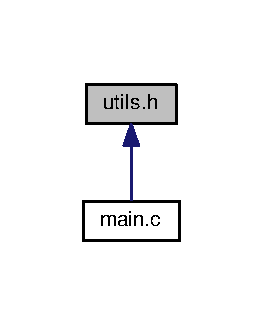
\includegraphics[width=126pt]{utils_8h__dep__incl}
\end{center}
\end{figure}
\subsection*{Functions}
\begin{DoxyCompactItemize}
\item 
void \hyperlink{utils_8h_a9d7e8af417b6d543da691e9c0e2f6f9f}{clear\+Screen} ()
\item 
void \hyperlink{utils_8h_a821efd1de9257a6ac8bce69ecc1e5dfc}{init\+Matrix} (char tabuleiro\mbox{[}$\,$\mbox{]}\mbox{[}10\mbox{]})
\item 
void \hyperlink{utils_8h_a4898a09411ad503295bdbe640b05dd10}{print\+About} ()
\item 
void \hyperlink{utils_8h_aa4f7464685f4b851ed78ed3a99254372}{print\+Align} (int space, char $\ast$string)
\item 
void \hyperlink{utils_8h_a1ea6231221c4e03a66d89d0c38aa71cc}{print\+Battleship} ()
\item 
void \hyperlink{utils_8h_a087a2b7743093438ffebaedb708e3283}{print\+Menu1} ()
\item 
void \hyperlink{utils_8h_a4f2acb39a12d6c7570980ae92ec9befc}{print\+Menu2} ()
\item 
const char $\ast$ \hyperlink{utils_8h_afbbac206745f181d052cd054256405fb}{direction\+Message} (char direction)
\item 
const char $\ast$ \hyperlink{utils_8h_aa6fe75334720e315d3182069c55e3a68}{ship\+Name} (char ship)
\item 
const int \hyperlink{utils_8h_a35e15ea010d1f6dc8f27c9c574dec78e}{get\+Ship\+Size} (char ship)
\item 
int \hyperlink{utils_8h_a8358f6f92781e2826cbcbbeb4b091ee5}{check\+Threshold} (char line, int col)
\item 
int \hyperlink{utils_8h_ad6cbd447e86b9eec5fe75e15370b3326}{check\+Coordenate} (char ship\+Type, char line, int col, char direction, char tabuleiro\mbox{[}$\,$\mbox{]}\mbox{[}10\mbox{]})
\item 
void \hyperlink{utils_8h_a362f75fd778db4d81e30c8e0f04495eb}{read\+Coordenate} (char $\ast$line, int $\ast$col)
\item 
void \hyperlink{utils_8h_a191c68084d72322fdfb77df4f0fefb4d}{check\+Shot} (char jogadas\mbox{[}$\,$\mbox{]}\mbox{[}10\mbox{]}, char tabuleiro\+Adversario\mbox{[}$\,$\mbox{]}\mbox{[}10\mbox{]}, char $\ast$nome\+Jogador, char $\ast$nome\+Adversario, int line, int col)
\item 
void \hyperlink{utils_8h_abec49bb0c079b81567289b409b10e4d9}{display\+Game\+Info} (char $\ast$nome\+Jogador1, char jogadas1\mbox{[}$\,$\mbox{]}\mbox{[}10\mbox{]}, char $\ast$nome\+Jogador2, char jogadas2\mbox{[}$\,$\mbox{]}\mbox{[}10\mbox{]})
\item 
void \hyperlink{utils_8h_ad3e46e8d515b2646486f391643333ed4}{display\+Game\+Player} (char $\ast$nome\+Jogador, char tabuleiro\mbox{[}$\,$\mbox{]}\mbox{[}10\mbox{]})
\item 
int \hyperlink{utils_8h_af4cf37339d3d98a2cbe99929874d9f02}{is\+End\+Game} (char jogadas\mbox{[}$\,$\mbox{]}\mbox{[}10\mbox{]})
\item 
void \hyperlink{utils_8h_a53aa17bcb66102859da0e09b78412911}{give\+Shot} (char jogadas\mbox{[}$\,$\mbox{]}\mbox{[}10\mbox{]}, char tabuleiro\+Adversario\mbox{[}$\,$\mbox{]}\mbox{[}10\mbox{]}, char $\ast$nome\+Jogador, char $\ast$nome\+Adversario)
\item 
void \hyperlink{utils_8h_a916e66ee495d0e5ac7d061cb882381f9}{give\+Random\+Shot} (char jogadas\mbox{[}$\,$\mbox{]}\mbox{[}10\mbox{]}, char tabuleiro\+Adversario\mbox{[}$\,$\mbox{]}\mbox{[}10\mbox{]}, char $\ast$nome\+Jogador, char $\ast$nome\+Adversario)
\item 
void \hyperlink{utils_8h_a92c29996f0bd795ae58310f30ba24466}{put\+Ship} (char ship\+Type, char line, int col, char direction, char tabuleiro\mbox{[}$\,$\mbox{]}\mbox{[}10\mbox{]})
\item 
void \hyperlink{utils_8h_a8dbfb8ff4e945c557e1baa84ca1c39fa}{put\+Ships} (char $\ast$nome\+Jogador, char tabuleiro\mbox{[}$\,$\mbox{]}\mbox{[}10\mbox{]})
\item 
void \hyperlink{utils_8h_ac2fd4847b2382dbddfea8eb84c01cdad}{put\+Ships\+C\+OM} (char tabuleiro\mbox{[}$\,$\mbox{]}\mbox{[}10\mbox{]})
\item 
void \hyperlink{utils_8h_a450dd23155e8a975d341985f105342c3}{print\+Resultados} (char $\ast$nome\+Jogador, char jogadas\mbox{[}$\,$\mbox{]}\mbox{[}10\mbox{]}, char tabuleiro\mbox{[}$\,$\mbox{]}\mbox{[}10\mbox{]})
\end{DoxyCompactItemize}


\subsection{Function Documentation}
\mbox{\Hypertarget{utils_8h_ad6cbd447e86b9eec5fe75e15370b3326}\label{utils_8h_ad6cbd447e86b9eec5fe75e15370b3326}} 
\index{utils.\+h@{utils.\+h}!check\+Coordenate@{check\+Coordenate}}
\index{check\+Coordenate@{check\+Coordenate}!utils.\+h@{utils.\+h}}
\subsubsection{\texorpdfstring{check\+Coordenate()}{checkCoordenate()}}
{\footnotesize\ttfamily int check\+Coordenate (\begin{DoxyParamCaption}\item[{char}]{ship\+Type,  }\item[{char}]{line,  }\item[{int}]{col,  }\item[{char}]{direction,  }\item[{char}]{tabuleiro\mbox{[}$\,$\mbox{]}\mbox{[}10\mbox{]} }\end{DoxyParamCaption})}

Verifica se a coordenada é válida para inserção de uma embarcação no tabuleiro


\begin{DoxyParams}{Parameters}
{\em ship\+Type} & Tipo de embarcação \\
\hline
{\em line} & Linha da matriz \\
\hline
{\em col} & Coluna da matriz \\
\hline
{\em direction} & Direção do posicionamento da embarcação \\
\hline
{\em tabuleiro} & Tabuleiro do jogo \\
\hline
\end{DoxyParams}
\begin{DoxyReturn}{Returns}
1 se a coordenada é válido, 0 caso contrário
\end{DoxyReturn}
Verifica se a coordenada juntamente com a direção são válidas para inserção de uma embarcação no tabuleiro


\begin{DoxyParams}{Parameters}
{\em ship\+Type} & Tipo de embarcação \\
\hline
{\em line} & Linha da matriz \\
\hline
{\em col} & Coluna da matriz \\
\hline
{\em direction} & Direção do posicionamento da embarcação \\
\hline
{\em tabuleiro} & Tabuleiro do jogo \\
\hline
\end{DoxyParams}
\begin{DoxyReturn}{Returns}
1 se a coordenada é válida, 0 caso contrário 
\end{DoxyReturn}


Definition at line 168 of file utils.\+c.


\begin{DoxyCode}
168                                                                                             \{
169     \textcolor{keywordtype}{int} intLine = (int)line-65;
170     \textcolor{comment}{/* Verifico:}
171 \textcolor{comment}{     * - se é uma coordenada dentro da matriz}
172 \textcolor{comment}{     * - se a letra informada para a direção é válida}
173 \textcolor{comment}{     * - se a direção e a coordenada ficam dentro da matriz}
174 \textcolor{comment}{    */}
175     \textcolor{keywordflow}{if}(!\hyperlink{utils_8c_aca751d22e44a1f046b2f3b14fecc84a6}{checkThreshold}(intLine, col) 
176         || !(direction == \textcolor{charliteral}{'W'} || direction == \textcolor{charliteral}{'S'} || direction == \textcolor{charliteral}{'A'} || direction == \textcolor{charliteral}{'D'})
177         || (direction == \textcolor{charliteral}{'W'} && (intLine - \hyperlink{utils_8c_a35e15ea010d1f6dc8f27c9c574dec78e}{getShipSize}(shipType) < 0))
178         || (direction == \textcolor{charliteral}{'S'} && (intLine + \hyperlink{utils_8c_a35e15ea010d1f6dc8f27c9c574dec78e}{getShipSize}(shipType) > 10))
179         || (direction == \textcolor{charliteral}{'A'} && (col - \hyperlink{utils_8c_a35e15ea010d1f6dc8f27c9c574dec78e}{getShipSize}(shipType) < 0))
180         || (direction == \textcolor{charliteral}{'D'} && (col + \hyperlink{utils_8c_a35e15ea010d1f6dc8f27c9c574dec78e}{getShipSize}(shipType) > 10)))\{
181         \textcolor{keywordflow}{return} 0;
182     \}
183 
184     \textcolor{comment}{// Verifico se as posições em que a embarcação será colocada estão livres}
185     \textcolor{keywordflow}{switch}(direction)\{
186         \textcolor{keywordflow}{case} \textcolor{charliteral}{'W'}:
187             \textcolor{comment}{//"Para Cima"}
188             \textcolor{keywordflow}{for}(\textcolor{keywordtype}{int} i = intLine; i > (intLine - \hyperlink{utils_8c_a35e15ea010d1f6dc8f27c9c574dec78e}{getShipSize}(shipType)); i--)\{
189                 \textcolor{keywordflow}{if}(tabuleiro[i][col] != \textcolor{charliteral}{'.'})\{
190                     \textcolor{keywordflow}{return} 0;
191                 \}
192             \}
193             \textcolor{keywordflow}{break};
194         \textcolor{keywordflow}{case} \textcolor{charliteral}{'S'}:
195             \textcolor{comment}{//"Para Baixo"}
196             \textcolor{keywordflow}{for}(\textcolor{keywordtype}{int} i = intLine; i < (intLine + \hyperlink{utils_8c_a35e15ea010d1f6dc8f27c9c574dec78e}{getShipSize}(shipType)); i++)\{
197                 \textcolor{keywordflow}{if}(tabuleiro[i][col] != \textcolor{charliteral}{'.'})\{
198                     \textcolor{keywordflow}{return} 0;
199                 \}
200             \}
201             \textcolor{keywordflow}{break};
202         \textcolor{keywordflow}{case} \textcolor{charliteral}{'D'}:
203             \textcolor{comment}{//"Para Direita"}
204             \textcolor{keywordflow}{for}(\textcolor{keywordtype}{int} i = col; i < (col + \hyperlink{utils_8c_a35e15ea010d1f6dc8f27c9c574dec78e}{getShipSize}(shipType)); i++)\{
205                 \textcolor{keywordflow}{if}(tabuleiro[intLine][i] != \textcolor{charliteral}{'.'})\{
206                     \textcolor{keywordflow}{return} 0;
207                 \}
208             \}
209             \textcolor{keywordflow}{break};
210         \textcolor{keywordflow}{case} \textcolor{charliteral}{'A'}:
211             \textcolor{comment}{//"Para Esquerda"}
212             \textcolor{keywordflow}{for}(\textcolor{keywordtype}{int} i = col; i > (col - \hyperlink{utils_8c_a35e15ea010d1f6dc8f27c9c574dec78e}{getShipSize}(shipType)); i--)\{
213                 \textcolor{keywordflow}{if}(tabuleiro[intLine][i] != \textcolor{charliteral}{'.'})\{
214                     \textcolor{keywordflow}{return} 0;
215                 \}
216             \}
217             \textcolor{keywordflow}{break};
218     \}
219 
220     \textcolor{keywordflow}{return} 1;
221 \}
\end{DoxyCode}
\mbox{\Hypertarget{utils_8h_a191c68084d72322fdfb77df4f0fefb4d}\label{utils_8h_a191c68084d72322fdfb77df4f0fefb4d}} 
\index{utils.\+h@{utils.\+h}!check\+Shot@{check\+Shot}}
\index{check\+Shot@{check\+Shot}!utils.\+h@{utils.\+h}}
\subsubsection{\texorpdfstring{check\+Shot()}{checkShot()}}
{\footnotesize\ttfamily void check\+Shot (\begin{DoxyParamCaption}\item[{char}]{jogadas\mbox{[}$\,$\mbox{]}\mbox{[}10\mbox{]},  }\item[{char}]{tabuleiro\+Adversario\mbox{[}$\,$\mbox{]}\mbox{[}10\mbox{]},  }\item[{char $\ast$}]{nome\+Jogador,  }\item[{char $\ast$}]{nome\+Adversario,  }\item[{int}]{line,  }\item[{int}]{col }\end{DoxyParamCaption})}

Verifica o resultado de uma jogada (disparo) da batalha naval


\begin{DoxyParams}{Parameters}
{\em jogadas} & Jogadas realizadas pelo jogador até o momento. \\
\hline
{\em tabuleiro\+Adversario} & Tabuleiro do adversário \\
\hline
{\em nome\+Jogador} & Nome do jogador \\
\hline
{\em nome\+Adversario} & Nome do adversário \\
\hline
\end{DoxyParams}


Definition at line 254 of file utils.\+c.


\begin{DoxyCode}
254                                                                                                            
                         \{
255     \hyperlink{utils_8c_a9d7e8af417b6d543da691e9c0e2f6f9f}{clearScreen}();
256     \hyperlink{utils_8c_a1ea6231221c4e03a66d89d0c38aa71cc}{printBattleship}();
257     printf(\textcolor{stringliteral}{"\(\backslash\)n\(\backslash\)n"});
258 
259     printf(\textcolor{stringliteral}{"Resultado do disparo realizado por: %s\(\backslash\)n\(\backslash\)n"}, nomeJogador);
260 
261     printf(\textcolor{stringliteral}{"*****************************************************************\(\backslash\)n"});
262     \textcolor{comment}{// Verifico onde o disparo acertou e atribuo o indicador}
263     \textcolor{keywordflow}{if}(tabuleiroAdversario[line][col] == \textcolor{charliteral}{'.'})\{
264         jogadas[line][col] = \textcolor{charliteral}{'O'};
265         printf(\textcolor{stringliteral}{"* Água! \(\backslash\)n"});
266     \}\textcolor{keywordflow}{else}\{
267         printf(\textcolor{stringliteral}{"* Fogo! \(\backslash\)n"});
268         jogadas[line][col] = \textcolor{charliteral}{'X'};
269 
270         \textcolor{keywordtype}{char} shipType = tabuleiroAdversario[line][col]; \textcolor{comment}{// Guardo o tipo de embarcação atingida}
271         \textcolor{keywordtype}{int} contHits = 0; \textcolor{comment}{// Quantas vezes essa embarcação foi atingida}
272 
273         \textcolor{comment}{// Verifico se minha embarcação afundou}
274         \textcolor{keywordflow}{for}(\textcolor{keywordtype}{int} i = 0; i < 10; i ++)\{
275             \textcolor{keywordflow}{for}(\textcolor{keywordtype}{int} j = 0; j < 10; j++)\{
276                 \textcolor{comment}{// Se há um disparo para minha embarcação, acumulo o número de vezes que ela foi acertada}
277                 \textcolor{keywordflow}{if}(jogadas[i][j] == \textcolor{charliteral}{'X'} && tabuleiroAdversario[i][j] == shipType)\{
278                     contHits++;
279                 \}
280             \}
281         \}
282 
283         \textcolor{comment}{// Se acertei o número de vezes igual ao tamanho dela, significa que afundei a embarcação}
284         \textcolor{keywordflow}{if}(contHits == \hyperlink{utils_8c_a35e15ea010d1f6dc8f27c9c574dec78e}{getShipSize}(shipType))\{
285             printf(\textcolor{stringliteral}{"* %s: Afundou %s %s!\(\backslash\)n"}, nomeAdversario, shipType == \textcolor{charliteral}{'N'} ? \textcolor{stringliteral}{"minha"} : \textcolor{stringliteral}{"meu"}, 
      \hyperlink{utils_8c_aa6fe75334720e315d3182069c55e3a68}{shipName}(shipType));
286 
287             \textcolor{comment}{// Mostro no tabuleiro minha embarcação}
288             \textcolor{keywordflow}{for}(\textcolor{keywordtype}{int} i = 0; i < 10; i ++)\{
289                 \textcolor{keywordflow}{for}(\textcolor{keywordtype}{int} j = 0; j < 10; j++)\{
290                     \textcolor{comment}{// Procuro as posições da embarcação afundada e coloco a sigla dela para ser mostrada}
291                     \textcolor{keywordflow}{if}(tabuleiroAdversario[i][j] == shipType)\{
292                         jogadas[i][j] = shipType;
293                     \}
294                 \}
295             \}
296         \}
297     \}
298     printf(\textcolor{stringliteral}{"*****************************************************************\(\backslash\)n"});
299     printf(\textcolor{stringliteral}{"\(\backslash\)n\(\backslash\)n\(\backslash\)n"});
300 \}
\end{DoxyCode}
\mbox{\Hypertarget{utils_8h_a8358f6f92781e2826cbcbbeb4b091ee5}\label{utils_8h_a8358f6f92781e2826cbcbbeb4b091ee5}} 
\index{utils.\+h@{utils.\+h}!check\+Threshold@{check\+Threshold}}
\index{check\+Threshold@{check\+Threshold}!utils.\+h@{utils.\+h}}
\subsubsection{\texorpdfstring{check\+Threshold()}{checkThreshold()}}
{\footnotesize\ttfamily int check\+Threshold (\begin{DoxyParamCaption}\item[{char}]{line,  }\item[{int}]{col }\end{DoxyParamCaption})}

Verifica se a coordenada é válidas para inserção de uma embarcação no tabuleiro


\begin{DoxyParams}{Parameters}
{\em line} & Linha da matriz \\
\hline
{\em col} & Coluna da matriz \\
\hline
\end{DoxyParams}
\begin{DoxyReturn}{Returns}
1 se a coordenada é válida, 0 caso contrário 
\end{DoxyReturn}
\mbox{\Hypertarget{utils_8h_a9d7e8af417b6d543da691e9c0e2f6f9f}\label{utils_8h_a9d7e8af417b6d543da691e9c0e2f6f9f}} 
\index{utils.\+h@{utils.\+h}!clear\+Screen@{clear\+Screen}}
\index{clear\+Screen@{clear\+Screen}!utils.\+h@{utils.\+h}}
\subsubsection{\texorpdfstring{clear\+Screen()}{clearScreen()}}
{\footnotesize\ttfamily void clear\+Screen (\begin{DoxyParamCaption}{ }\end{DoxyParamCaption})}

Limpa a tela do console 

Definition at line 18 of file utils.\+c.


\begin{DoxyCode}
18                   \{
19   system(\textcolor{stringliteral}{"@cls||clear"});
20 \}
\end{DoxyCode}
\mbox{\Hypertarget{utils_8h_afbbac206745f181d052cd054256405fb}\label{utils_8h_afbbac206745f181d052cd054256405fb}} 
\index{utils.\+h@{utils.\+h}!direction\+Message@{direction\+Message}}
\index{direction\+Message@{direction\+Message}!utils.\+h@{utils.\+h}}
\subsubsection{\texorpdfstring{direction\+Message()}{directionMessage()}}
{\footnotesize\ttfamily const char$\ast$ direction\+Message (\begin{DoxyParamCaption}\item[{char}]{direction }\end{DoxyParamCaption})}

Retorna a mensagem correspondende à cada direção 

Definition at line 98 of file utils.\+c.


\begin{DoxyCode}
98                                              \{
99     \textcolor{keywordflow}{switch}(direction)\{
100         \textcolor{keywordflow}{case} \textcolor{charliteral}{'W'}:
101             \textcolor{keywordflow}{return} \textcolor{stringliteral}{"Para Cima"};
102         \textcolor{keywordflow}{case} \textcolor{charliteral}{'S'}:
103             \textcolor{keywordflow}{return} \textcolor{stringliteral}{"Para Baixo"};
104         \textcolor{keywordflow}{case} \textcolor{charliteral}{'D'}:
105             \textcolor{keywordflow}{return} \textcolor{stringliteral}{"Para Direita"};
106         \textcolor{keywordflow}{case} \textcolor{charliteral}{'A'}:
107             \textcolor{keywordflow}{return} \textcolor{stringliteral}{"Para Esquerda"};
108     \} 
109 \}
\end{DoxyCode}
\mbox{\Hypertarget{utils_8h_abec49bb0c079b81567289b409b10e4d9}\label{utils_8h_abec49bb0c079b81567289b409b10e4d9}} 
\index{utils.\+h@{utils.\+h}!display\+Game\+Info@{display\+Game\+Info}}
\index{display\+Game\+Info@{display\+Game\+Info}!utils.\+h@{utils.\+h}}
\subsubsection{\texorpdfstring{display\+Game\+Info()}{displayGameInfo()}}
{\footnotesize\ttfamily void display\+Game\+Info (\begin{DoxyParamCaption}\item[{char $\ast$}]{nome\+Jogador1,  }\item[{char}]{jogadas1\mbox{[}$\,$\mbox{]}\mbox{[}10\mbox{]},  }\item[{char $\ast$}]{nome\+Jogador2,  }\item[{char}]{jogadas2\mbox{[}$\,$\mbox{]}\mbox{[}10\mbox{]} }\end{DoxyParamCaption})}

Mostra as informações de duas matrizes lado a lado com o nome dos jogadores. Exemplo\+: Player $\vert$ Computer 0 1 2 3 4 5 6 7 8 9 $\vert$ 0 1 2 3 4 5 6 7 8 9 A $\vert$\+P$\vert$ $\vert$ $\vert$ $\vert$ $\vert$ $\vert$ $\vert$ $\vert$ $\vert$ $\vert$ $\vert$ A $\vert$ $\vert$ $\vert$ $\vert$ $\vert$ $\vert$ $\vert$ $\vert$ $\vert$ $\vert$ $\vert$ B $\vert$\+P$\vert$ $\vert$ $\vert$ $\vert$ $\vert$ $\vert$ $\vert$ $\vert$ $\vert$ $\vert$ $\vert$ B $\vert$ $\vert$ $\vert$ $\vert$ $\vert$ $\vert$ $\vert$ $\vert$ $\vert$ $\vert$ $\vert$ C $\vert$\+P$\vert$ $\vert$ $\vert$ $\vert$ $\vert$ $\vert$ $\vert$ $\vert$ $\vert$ $\vert$ $\vert$ C $\vert$ $\vert$ $\vert$ $\vert$ $\vert$ $\vert$ $\vert$\+O$\vert$ $\vert$ $\vert$ $\vert$ D $\vert$\+P$\vert$ $\vert$ $\vert$ $\vert$ $\vert$ $\vert$ $\vert$ $\vert$ $\vert$ $\vert$ $\vert$ D $\vert$ $\vert$ $\vert$x$\vert$ $\vert$ $\vert$ $\vert$ $\vert$ $\vert$ $\vert$ $\vert$ E $\vert$\+P$\vert$ $\vert$ $\vert$ $\vert$ $\vert$ $\vert$ $\vert$ $\vert$ $\vert$ $\vert$ $\vert$ E $\vert$ $\vert$ $\vert$ $\vert$ $\vert$ $\vert$ $\vert$ $\vert$ $\vert$ $\vert$ $\vert$ F $\vert$ $\vert$ $\vert$ $\vert$ $\vert$ $\vert$ $\vert$ $\vert$ $\vert$ $\vert$ $\vert$ $\vert$ F $\vert$ $\vert$ $\vert$ $\vert$ $\vert$\+O$\vert$ $\vert$ $\vert$ $\vert$ $\vert$ $\vert$ G $\vert$ $\vert$ $\vert$ $\vert$ $\vert$ $\vert$ $\vert$ $\vert$ $\vert$ $\vert$ $\vert$ $\vert$ G $\vert$ $\vert$ $\vert$ $\vert$ $\vert$ $\vert$ $\vert$ $\vert$ $\vert$ $\vert$ $\vert$ H $\vert$ $\vert$ $\vert$ $\vert$ $\vert$ $\vert$ $\vert$ $\vert$ $\vert$ $\vert$ $\vert$ $\vert$ H $\vert$ $\vert$\+O$\vert$ $\vert$ $\vert$ $\vert$ $\vert$\+O$\vert$ $\vert$ $\vert$ $\vert$ I $\vert$ $\vert$ $\vert$ $\vert$ $\vert$ $\vert$ $\vert$ $\vert$ $\vert$ $\vert$ $\vert$ $\vert$ I $\vert$ $\vert$ $\vert$ $\vert$ $\vert$ $\vert$ $\vert$ $\vert$ $\vert$ $\vert$ $\vert$ J $\vert$ $\vert$ $\vert$ $\vert$ $\vert$ $\vert$ $\vert$ $\vert$ $\vert$ $\vert$ $\vert$ $\vert$ J $\vert$ $\vert$ $\vert$ $\vert$ $\vert$ $\vert$ $\vert$ $\vert$ $\vert$ $\vert$ $\vert$


\begin{DoxyParams}{Parameters}
{\em nome\+Jogador1} & Nome do jogador 1 \\
\hline
{\em jogadas1} & Tabuleiro de jogadas do jogador 1 \\
\hline
{\em nome\+Jogador2} & Nome do jogador 2 \\
\hline
{\em jogadas2} & Tabuleiro de jogadas do jogador 2\\
\hline
\end{DoxyParams}
Mostra as informações dos tabuleiros lado a lado de dois jogadores com os seus respectivos nomes. Exemplo\+: Player $\vert$ Computer 0 1 2 3 4 5 6 7 8 9 $\vert$ 0 1 2 3 4 5 6 7 8 9 A $\vert$\+P$\vert$ $\vert$ $\vert$ $\vert$ $\vert$ $\vert$ $\vert$ $\vert$ $\vert$ $\vert$ $\vert$ A $\vert$ $\vert$ $\vert$ $\vert$ $\vert$ $\vert$ $\vert$ $\vert$ $\vert$ $\vert$ $\vert$ B $\vert$\+P$\vert$ $\vert$ $\vert$ $\vert$ $\vert$ $\vert$ $\vert$ $\vert$ $\vert$ $\vert$ $\vert$ B $\vert$ $\vert$ $\vert$ $\vert$ $\vert$ $\vert$ $\vert$ $\vert$ $\vert$ $\vert$ $\vert$ C $\vert$\+P$\vert$ $\vert$ $\vert$ $\vert$ $\vert$ $\vert$ $\vert$ $\vert$ $\vert$ $\vert$ $\vert$ C $\vert$ $\vert$ $\vert$ $\vert$ $\vert$ $\vert$ $\vert$\+O$\vert$ $\vert$ $\vert$ $\vert$ D $\vert$\+P$\vert$ $\vert$ $\vert$ $\vert$ $\vert$ $\vert$ $\vert$ $\vert$ $\vert$ $\vert$ $\vert$ D $\vert$ $\vert$ $\vert$x$\vert$ $\vert$ $\vert$ $\vert$ $\vert$ $\vert$ $\vert$ $\vert$ E $\vert$\+P$\vert$ $\vert$ $\vert$ $\vert$ $\vert$ $\vert$ $\vert$ $\vert$ $\vert$ $\vert$ $\vert$ E $\vert$ $\vert$ $\vert$ $\vert$ $\vert$ $\vert$ $\vert$ $\vert$ $\vert$ $\vert$ $\vert$ F $\vert$ $\vert$ $\vert$ $\vert$ $\vert$ $\vert$ $\vert$ $\vert$ $\vert$ $\vert$ $\vert$ $\vert$ F $\vert$ $\vert$ $\vert$ $\vert$ $\vert$\+O$\vert$ $\vert$ $\vert$ $\vert$ $\vert$ $\vert$ G $\vert$ $\vert$ $\vert$ $\vert$ $\vert$ $\vert$ $\vert$ $\vert$ $\vert$ $\vert$ $\vert$ $\vert$ G $\vert$ $\vert$ $\vert$ $\vert$ $\vert$ $\vert$ $\vert$ $\vert$ $\vert$ $\vert$ $\vert$ H $\vert$ $\vert$ $\vert$ $\vert$ $\vert$ $\vert$ $\vert$ $\vert$ $\vert$ $\vert$ $\vert$ $\vert$ H $\vert$ $\vert$\+O$\vert$ $\vert$ $\vert$ $\vert$ $\vert$\+O$\vert$ $\vert$ $\vert$ $\vert$ I $\vert$ $\vert$ $\vert$ $\vert$ $\vert$ $\vert$ $\vert$ $\vert$ $\vert$ $\vert$ $\vert$ $\vert$ I $\vert$ $\vert$ $\vert$ $\vert$ $\vert$ $\vert$ $\vert$ $\vert$ $\vert$ $\vert$ $\vert$ J $\vert$ $\vert$ $\vert$ $\vert$ $\vert$ $\vert$ $\vert$ $\vert$ $\vert$ $\vert$ $\vert$ $\vert$ J $\vert$ $\vert$ $\vert$ $\vert$ $\vert$ $\vert$ $\vert$ $\vert$ $\vert$ $\vert$ $\vert$


\begin{DoxyParams}{Parameters}
{\em nome\+Jogador1} & Nome do jogador 1 \\
\hline
{\em jogadas1} & Tabuleiro de jogadas do jogador 1 \\
\hline
{\em nome\+Jogador2} & Nome do jogador 2 \\
\hline
{\em jogadas2} & Tabuleiro de jogadas do jogador 2 \\
\hline
\end{DoxyParams}


Definition at line 323 of file utils.\+c.


\begin{DoxyCode}
323                                                                                                       \{
324     \textcolor{keywordtype}{char} separador[] = \textcolor{stringliteral}{"     |   "};
325 
326     \textcolor{comment}{// Imprimo o cabeçalho}
327     \hyperlink{utils_8c_aa4f7464685f4b851ed78ed3a99254372}{printAlign}(41, nomeJogador1);
328     printf(\textcolor{stringliteral}{"%s"}, separador);
329     \hyperlink{utils_8c_aa4f7464685f4b851ed78ed3a99254372}{printAlign}(44, nomeJogador2);
330     printf(\textcolor{stringliteral}{"\(\backslash\)n"});
331 
332     \textcolor{keywordflow}{for}(\textcolor{keywordtype}{int} cont = 0; cont < 2; cont++)\{
333         printf(\textcolor{stringliteral}{" "});
334         \textcolor{keywordflow}{for} (\textcolor{keywordtype}{int} i = 0; i < 10; i++) \{
335             printf(\textcolor{stringliteral}{"   %i"}, i);
336         \}
337         \textcolor{keywordflow}{if}(!cont)\{
338             printf(\textcolor{stringliteral}{"%s"}, separador);
339         \}
340     \}
341     printf(\textcolor{stringliteral}{"\(\backslash\)n"});
342     
343     \textcolor{comment}{// Imprimo as linhas}
344     \textcolor{keywordflow}{for} (\textcolor{keywordtype}{int} i = 0; i < 10; i++) \{
345         \textcolor{comment}{// Imprime a letra}
346         printf(\textcolor{stringliteral}{"%c | "}, 65+i);
347 
348         \textcolor{comment}{// Imprime os valores do player1}
349         \textcolor{keywordflow}{for} (\textcolor{keywordtype}{int} j = 0; j < 10; j++) \{
350             printf(\textcolor{stringliteral}{"%c | "}, jogadas1[i][j]);
351         \}
352 
353         \textcolor{comment}{// Imprime a letra}
354         printf(\textcolor{stringliteral}{"  |   %c | "}, 65+i);
355         \textcolor{comment}{// Imprime os valores do player 2}
356         \textcolor{keywordflow}{for} (\textcolor{keywordtype}{int} j = 0; j < 10; j++) \{
357             printf(\textcolor{stringliteral}{"%c | "}, jogadas2[i][j]);
358         \}
359         printf(\textcolor{stringliteral}{"\(\backslash\)n"});
360     \}
361 \}
\end{DoxyCode}
\mbox{\Hypertarget{utils_8h_ad3e46e8d515b2646486f391643333ed4}\label{utils_8h_ad3e46e8d515b2646486f391643333ed4}} 
\index{utils.\+h@{utils.\+h}!display\+Game\+Player@{display\+Game\+Player}}
\index{display\+Game\+Player@{display\+Game\+Player}!utils.\+h@{utils.\+h}}
\subsubsection{\texorpdfstring{display\+Game\+Player()}{displayGamePlayer()}}
{\footnotesize\ttfamily void display\+Game\+Player (\begin{DoxyParamCaption}\item[{char $\ast$}]{nome\+Jogador,  }\item[{char}]{tabuleiro\mbox{[}$\,$\mbox{]}\mbox{[}10\mbox{]} }\end{DoxyParamCaption})}

Mostra as informações do tabuleiro do jogador com os seu respectivo nome. Exemplo\+: Player 0 1 2 3 4 5 6 7 8 9 A $\vert$\+P$\vert$ $\vert$ $\vert$ $\vert$ $\vert$ $\vert$ $\vert$ $\vert$ $\vert$ $\vert$ B $\vert$\+P$\vert$ $\vert$ $\vert$ $\vert$ $\vert$ $\vert$ $\vert$ $\vert$ $\vert$ $\vert$ C $\vert$\+P$\vert$ $\vert$ $\vert$ $\vert$ $\vert$ $\vert$ $\vert$ $\vert$ $\vert$ $\vert$ D $\vert$\+P$\vert$ $\vert$ $\vert$ $\vert$ $\vert$ $\vert$ $\vert$ $\vert$ $\vert$ $\vert$ E $\vert$\+P$\vert$ $\vert$ $\vert$ $\vert$ $\vert$ $\vert$ $\vert$ $\vert$ $\vert$ $\vert$ F $\vert$ $\vert$ $\vert$ $\vert$ $\vert$ $\vert$ $\vert$ $\vert$ $\vert$ $\vert$ $\vert$ G $\vert$ $\vert$ $\vert$ $\vert$ $\vert$\+N$\vert$\+N$\vert$\+N$\vert$ $\vert$ $\vert$ $\vert$ H $\vert$ $\vert$ $\vert$ $\vert$ $\vert$ $\vert$ $\vert$ $\vert$ $\vert$ $\vert$ $\vert$ I $\vert$ $\vert$ $\vert$ $\vert$ $\vert$ $\vert$ $\vert$ $\vert$ $\vert$ $\vert$ $\vert$ J $\vert$ $\vert$ $\vert$ $\vert$ $\vert$ $\vert$ $\vert$ $\vert$ $\vert$ $\vert$ $\vert$


\begin{DoxyParams}{Parameters}
{\em nome\+Jogador} & Nome do jogador \\
\hline
{\em tabuleiro} & Tabuleiro do jogador \\
\hline
\end{DoxyParams}


Definition at line 382 of file utils.\+c.


\begin{DoxyCode}
382                                                                \{
383     \textcolor{keywordtype}{char} separador[] = \textcolor{stringliteral}{"     |   "};
384 
385     \textcolor{comment}{// Imprimo o cabeçalho}
386     \hyperlink{utils_8c_aa4f7464685f4b851ed78ed3a99254372}{printAlign}(41, nomeJogador);
387     printf(\textcolor{stringliteral}{"\(\backslash\)n"});
388     
389     printf(\textcolor{stringliteral}{" "});
390     \textcolor{keywordflow}{for} (\textcolor{keywordtype}{int} i = 0; i < 10; i++) \{
391         printf(\textcolor{stringliteral}{"   %i"}, i);
392     \}
393     printf(\textcolor{stringliteral}{"\(\backslash\)n"});
394     
395     \textcolor{comment}{// Imprimo as linhas}
396     \textcolor{keywordflow}{for} (\textcolor{keywordtype}{int} i = 0; i < 10; i++) \{
397         \textcolor{comment}{// Imprime a letra}
398         printf(\textcolor{stringliteral}{"%c | "}, 65+i);
399 
400         \textcolor{comment}{// Imprime os valores do jogador}
401         \textcolor{keywordflow}{for} (\textcolor{keywordtype}{int} j = 0; j < 10; j++) \{
402             printf(\textcolor{stringliteral}{"%c | "}, tabuleiro[i][j]);
403         \}
404         printf(\textcolor{stringliteral}{"\(\backslash\)n"});
405     \}
406 \}
\end{DoxyCode}
\mbox{\Hypertarget{utils_8h_a35e15ea010d1f6dc8f27c9c574dec78e}\label{utils_8h_a35e15ea010d1f6dc8f27c9c574dec78e}} 
\index{utils.\+h@{utils.\+h}!get\+Ship\+Size@{get\+Ship\+Size}}
\index{get\+Ship\+Size@{get\+Ship\+Size}!utils.\+h@{utils.\+h}}
\subsubsection{\texorpdfstring{get\+Ship\+Size()}{getShipSize()}}
{\footnotesize\ttfamily const int get\+Ship\+Size (\begin{DoxyParamCaption}\item[{char}]{ship }\end{DoxyParamCaption})}

Retorna o tamanho da embarcação de acordo com a sigla 

Definition at line 132 of file utils.\+c.


\begin{DoxyCode}
132                                 \{
133     \textcolor{keywordflow}{switch}(ship)\{
134         \textcolor{keywordflow}{case} \textcolor{charliteral}{'P'}:
135             \textcolor{keywordflow}{return} 5;
136         \textcolor{keywordflow}{case} \textcolor{charliteral}{'N'}:
137             \textcolor{keywordflow}{return} 4;
138         \textcolor{keywordflow}{case} \textcolor{charliteral}{'C'}:
139             \textcolor{keywordflow}{return} 3;
140         \textcolor{keywordflow}{case} \textcolor{charliteral}{'S'}:
141             \textcolor{keywordflow}{return} 3;
142         \textcolor{keywordflow}{case} \textcolor{charliteral}{'D'}:
143             \textcolor{keywordflow}{return} 2;
144     \}
145 \}
\end{DoxyCode}
\mbox{\Hypertarget{utils_8h_a916e66ee495d0e5ac7d061cb882381f9}\label{utils_8h_a916e66ee495d0e5ac7d061cb882381f9}} 
\index{utils.\+h@{utils.\+h}!give\+Random\+Shot@{give\+Random\+Shot}}
\index{give\+Random\+Shot@{give\+Random\+Shot}!utils.\+h@{utils.\+h}}
\subsubsection{\texorpdfstring{give\+Random\+Shot()}{giveRandomShot()}}
{\footnotesize\ttfamily void give\+Random\+Shot (\begin{DoxyParamCaption}\item[{char}]{jogadas\mbox{[}$\,$\mbox{]}\mbox{[}10\mbox{]},  }\item[{char}]{tabuleiro\+Adversario\mbox{[}$\,$\mbox{]}\mbox{[}10\mbox{]},  }\item[{char $\ast$}]{nome\+Jogador,  }\item[{char $\ast$}]{nome\+Adversario }\end{DoxyParamCaption})}

A máquina realiza uma jogada (disparo) da batalha naval


\begin{DoxyParams}{Parameters}
{\em jogadas} & Jogadas realizadas pelo jogador até o momento. \\
\hline
{\em tabuleiro\+Adversario} & Tabuleiro do adversário \\
\hline
{\em nome\+Jogador} & Nome do jogador \\
\hline
{\em nome\+Adversario} & Nome do adversário \\
\hline
\end{DoxyParams}


Definition at line 492 of file utils.\+c.


\begin{DoxyCode}
492                                                                                                            
           \{
493     \textcolor{keywordtype}{int} col, line;
494     
495     \textcolor{keywordflow}{do}\{
496         srand(time(NULL));
497         line = rand() % 10;
498         col = rand() % 10;
499         
500         \textcolor{keywordflow}{if}(jogadas[line][col] == \textcolor{charliteral}{'.'})\{
501             \textcolor{keywordflow}{break};
502         \}
503     \}\textcolor{keywordflow}{while}(1);
504 
505     \hyperlink{utils_8c_a191c68084d72322fdfb77df4f0fefb4d}{checkShot}(jogadas, tabuleiroAdversario, nomeJogador, nomeAdversario, line, col);
506 \}
\end{DoxyCode}
\mbox{\Hypertarget{utils_8h_a53aa17bcb66102859da0e09b78412911}\label{utils_8h_a53aa17bcb66102859da0e09b78412911}} 
\index{utils.\+h@{utils.\+h}!give\+Shot@{give\+Shot}}
\index{give\+Shot@{give\+Shot}!utils.\+h@{utils.\+h}}
\subsubsection{\texorpdfstring{give\+Shot()}{giveShot()}}
{\footnotesize\ttfamily void give\+Shot (\begin{DoxyParamCaption}\item[{char}]{jogadas\mbox{[}$\,$\mbox{]}\mbox{[}10\mbox{]},  }\item[{char}]{tabuleiro\+Adversario\mbox{[}$\,$\mbox{]}\mbox{[}10\mbox{]},  }\item[{char $\ast$}]{nome\+Jogador,  }\item[{char $\ast$}]{nome\+Adversario }\end{DoxyParamCaption})}

Realiza uma jogada (disparo) da batalha naval por um jogador


\begin{DoxyParams}{Parameters}
{\em jogadas} & Jogadas realizadas pelo jogador até o momento. \\
\hline
{\em tabuleiro\+Adversario} & Tabuleiro do adversário \\
\hline
{\em nome\+Jogador} & Nome do jogador \\
\hline
{\em nome\+Adversario} & Nome do adversário \\
\hline
\end{DoxyParams}


Definition at line 464 of file utils.\+c.


\begin{DoxyCode}
464                                                                                                           \{
465     \textcolor{keywordtype}{int} col, intLine;
466     \textcolor{keywordtype}{char} line;
467 
468     \textcolor{comment}{// O programa solicita um disparo válido}
469     \textcolor{keywordflow}{do}\{
470         \hyperlink{utils_8c_a362f75fd778db4d81e30c8e0f04495eb}{readCoordenate}(&line, &col);
471 
472         intLine = (int)line-65;
473 
474         \textcolor{keywordflow}{if}(jogadas[intLine][col] == \textcolor{charliteral}{'.'})\{
475             \textcolor{keywordflow}{break};
476         \}\textcolor{keywordflow}{else}\{
477             printf(\textcolor{stringliteral}{"Essa coordenada já foi informada anteriormente. Tente novamente.\(\backslash\)n"});
478         \}       
479     \}\textcolor{keywordflow}{while}(1);
480 
481     \hyperlink{utils_8c_a191c68084d72322fdfb77df4f0fefb4d}{checkShot}(jogadas, tabuleiroAdversario, nomeJogador, nomeAdversario, intLine, col);
482 \}
\end{DoxyCode}
\mbox{\Hypertarget{utils_8h_a821efd1de9257a6ac8bce69ecc1e5dfc}\label{utils_8h_a821efd1de9257a6ac8bce69ecc1e5dfc}} 
\index{utils.\+h@{utils.\+h}!init\+Matrix@{init\+Matrix}}
\index{init\+Matrix@{init\+Matrix}!utils.\+h@{utils.\+h}}
\subsubsection{\texorpdfstring{init\+Matrix()}{initMatrix()}}
{\footnotesize\ttfamily void init\+Matrix (\begin{DoxyParamCaption}\item[{char}]{tabuleiro\mbox{[}$\,$\mbox{]}\mbox{[}10\mbox{]} }\end{DoxyParamCaption})}

Inicializo cada posição do tabuleiro do jogador com \textquotesingle{}.\textquotesingle{}


\begin{DoxyParams}{Parameters}
{\em tabuleiro} & Tabuleiro do jogador \\
\hline
\end{DoxyParams}


Definition at line 27 of file utils.\+c.


\begin{DoxyCode}
27                                      \{
28     \textcolor{keywordflow}{for} (\textcolor{keywordtype}{int} i = 0; i < 10; i++) \{      
29       \textcolor{keywordflow}{for} (\textcolor{keywordtype}{int} j = 0; j < 10; j++) \{
30         tabuleiro[i][j] = \textcolor{charliteral}{'.'};
31       \}      
32     \}
33 \}
\end{DoxyCode}
\mbox{\Hypertarget{utils_8h_af4cf37339d3d98a2cbe99929874d9f02}\label{utils_8h_af4cf37339d3d98a2cbe99929874d9f02}} 
\index{utils.\+h@{utils.\+h}!is\+End\+Game@{is\+End\+Game}}
\index{is\+End\+Game@{is\+End\+Game}!utils.\+h@{utils.\+h}}
\subsubsection{\texorpdfstring{is\+End\+Game()}{isEndGame()}}
{\footnotesize\ttfamily int is\+End\+Game (\begin{DoxyParamCaption}\item[{char}]{jogadas\mbox{[}$\,$\mbox{]}\mbox{[}10\mbox{]} }\end{DoxyParamCaption})}

Verifica se o jogo já acabou


\begin{DoxyParams}{Parameters}
{\em jogadas} & Tabuleiro de jogadas de algum jogador \\
\hline
\end{DoxyParams}
\begin{DoxyReturn}{Returns}
Retorna 1 se todas as embarcações foram afundadas, 0 caso contrário 
\end{DoxyReturn}


Definition at line 414 of file utils.\+c.


\begin{DoxyCode}
414                                  \{
415     \textcolor{keywordtype}{int} embarcacoesAfundadas = 0;
416 
417     \textcolor{comment}{// Verifico se todas as embarcações foram afundadas}
418     \textcolor{keywordflow}{for}(\textcolor{keywordtype}{int} i = 0; i < 5; i++)\{
419 
420         \textcolor{keywordtype}{char} shipType;
421 
422         \textcolor{keywordflow}{switch}(i)\{
423             \textcolor{keywordflow}{case} 0:
424                 shipType = \textcolor{charliteral}{'P'};
425                 \textcolor{keywordflow}{break};
426             \textcolor{keywordflow}{case} 1:
427                 shipType = \textcolor{charliteral}{'N'};
428                 \textcolor{keywordflow}{break};
429             \textcolor{keywordflow}{case} 2:
430                 shipType = \textcolor{charliteral}{'C'};
431                 \textcolor{keywordflow}{break};
432             \textcolor{keywordflow}{case} 3:
433                 shipType = \textcolor{charliteral}{'S'};
434                 \textcolor{keywordflow}{break};
435             \textcolor{keywordflow}{case} 4:
436                 shipType = \textcolor{charliteral}{'D'};
437                 \textcolor{keywordflow}{break};
438         \}
439 
440         \textcolor{comment}{// Se o tabuleiro contém a letra da embarcação significa que essa embarcação foi afundada}
441         \textcolor{keywordflow}{for}(\textcolor{keywordtype}{int} i = 0; i < 10; i++)\{
442             \textcolor{keywordflow}{for}(\textcolor{keywordtype}{int} j = 0; j < 10; j++)\{
443                 \textcolor{keywordflow}{if}(jogadas[i][j] == shipType)\{
444                     embarcacoesAfundadas++;
445                     i = j = 10;
446                     \textcolor{keywordflow}{break};
447                 \}
448             \}
449         \}
450     \}
451 
452     
453     \textcolor{keywordflow}{return} embarcacoesAfundadas == 5 ? 1 : 0;
454 \}
\end{DoxyCode}
\mbox{\Hypertarget{utils_8h_a4898a09411ad503295bdbe640b05dd10}\label{utils_8h_a4898a09411ad503295bdbe640b05dd10}} 
\index{utils.\+h@{utils.\+h}!print\+About@{print\+About}}
\index{print\+About@{print\+About}!utils.\+h@{utils.\+h}}
\subsubsection{\texorpdfstring{print\+About()}{printAbout()}}
{\footnotesize\ttfamily void print\+About (\begin{DoxyParamCaption}{ }\end{DoxyParamCaption})}

Mostra as informações sobre o jogo 

Definition at line 38 of file utils.\+c.


\begin{DoxyCode}
38                  \{
39     printf(\textcolor{stringliteral}{"**************************************************************\(\backslash\)n"});
40     printf(\textcolor{stringliteral}{"*Bem-vindo ao jogo de batalha naval! - Exemplo trabalho UFPR *\(\backslash\)n"});
41     printf(\textcolor{stringliteral}{"**************************************************************\(\backslash\)n"});
42     printf(\textcolor{stringliteral}{"\(\backslash\)n\(\backslash\)n\(\backslash\)n"});
43     printf(\textcolor{stringliteral}{"Esse exemplo foi desenvolvido por Jackson Antonio do Prado Lima.\(\backslash\)n\(\backslash\)n\(\backslash\)n"});
44 \}
\end{DoxyCode}
\mbox{\Hypertarget{utils_8h_aa4f7464685f4b851ed78ed3a99254372}\label{utils_8h_aa4f7464685f4b851ed78ed3a99254372}} 
\index{utils.\+h@{utils.\+h}!print\+Align@{print\+Align}}
\index{print\+Align@{print\+Align}!utils.\+h@{utils.\+h}}
\subsubsection{\texorpdfstring{print\+Align()}{printAlign()}}
{\footnotesize\ttfamily void print\+Align (\begin{DoxyParamCaption}\item[{int}]{space,  }\item[{char $\ast$}]{string }\end{DoxyParamCaption})}

Realiza o print de uma string de modo centralizado


\begin{DoxyParams}{Parameters}
{\em space} & Espaço máximo em que a string deverá ser centralizada \\
\hline
{\em string} & String a ser mostrada \\
\hline
\end{DoxyParams}


Definition at line 52 of file utils.\+c.


\begin{DoxyCode}
52                                         \{
53      \textcolor{keywordtype}{int} length = strlen(\textcolor{keywordtype}{string});
54 
55     printf (\textcolor{stringliteral}{"%*s%*c"}
56             ,((space - length) >> 1) + length \textcolor{comment}{// string length + padding spaces}
57             , \textcolor{keywordtype}{string}
58             , ((space - length) >> 1) + ((space - length) & 1) \textcolor{comment}{// tailing spaces}
59             , \textcolor{charliteral}{' '}
60     );
61 \}
\end{DoxyCode}
\mbox{\Hypertarget{utils_8h_a1ea6231221c4e03a66d89d0c38aa71cc}\label{utils_8h_a1ea6231221c4e03a66d89d0c38aa71cc}} 
\index{utils.\+h@{utils.\+h}!print\+Battleship@{print\+Battleship}}
\index{print\+Battleship@{print\+Battleship}!utils.\+h@{utils.\+h}}
\subsubsection{\texorpdfstring{print\+Battleship()}{printBattleship()}}
{\footnotesize\ttfamily void print\+Battleship (\begin{DoxyParamCaption}{ }\end{DoxyParamCaption})}

Mostra o nome do jogo de modo estilizado 

Definition at line 66 of file utils.\+c.


\begin{DoxyCode}
66                       \{
67     printf (\textcolor{stringliteral}{"XXXXX   XXXX  XXXXXX XXXXXX XX     XXXXXX  XXXXX XX  XX XX XXXX\(\backslash\)n"});
68     printf (\textcolor{stringliteral}{"XX  XX XX  XX   XX     XX   XX     XX     XX     XX  XX XX XX  XX\(\backslash\)n"});
69     printf (\textcolor{stringliteral}{"XXXXX  XX  XX   XX     XX   XX     XXXX    XXXX  XXXXXX XX XXXX\(\backslash\)n"}); 
70     printf (\textcolor{stringliteral}{"XX  XX XXXXXX   XX     XX   XX     XX         XX XX  XX XX XX\(\backslash\)n"});
71     printf (\textcolor{stringliteral}{"XXXXX  XX  XX   XX     XX   XXXXXX XXXXXX XXXXX  XX  XX XX XX\(\backslash\)n"}); 
72     printf (\textcolor{stringliteral}{"\(\backslash\)n\(\backslash\)n"});
73 \}
\end{DoxyCode}
\mbox{\Hypertarget{utils_8h_a087a2b7743093438ffebaedb708e3283}\label{utils_8h_a087a2b7743093438ffebaedb708e3283}} 
\index{utils.\+h@{utils.\+h}!print\+Menu1@{print\+Menu1}}
\index{print\+Menu1@{print\+Menu1}!utils.\+h@{utils.\+h}}
\subsubsection{\texorpdfstring{print\+Menu1()}{printMenu1()}}
{\footnotesize\ttfamily void print\+Menu1 (\begin{DoxyParamCaption}{ }\end{DoxyParamCaption})}

Mostra as opções de menu iniciais 

Definition at line 78 of file utils.\+c.


\begin{DoxyCode}
78                  \{
79     printf (\textcolor{stringliteral}{"Escolha uma opção:\(\backslash\)n"});
80     printf (\textcolor{stringliteral}{"1) Jogar\(\backslash\)n"});  
81     printf (\textcolor{stringliteral}{"2) Sobre o jogo\(\backslash\)n"});
82     printf (\textcolor{stringliteral}{"3) Sair\(\backslash\)n\(\backslash\)n"});
83 \}
\end{DoxyCode}
\mbox{\Hypertarget{utils_8h_a4f2acb39a12d6c7570980ae92ec9befc}\label{utils_8h_a4f2acb39a12d6c7570980ae92ec9befc}} 
\index{utils.\+h@{utils.\+h}!print\+Menu2@{print\+Menu2}}
\index{print\+Menu2@{print\+Menu2}!utils.\+h@{utils.\+h}}
\subsubsection{\texorpdfstring{print\+Menu2()}{printMenu2()}}
{\footnotesize\ttfamily void print\+Menu2 (\begin{DoxyParamCaption}{ }\end{DoxyParamCaption})}

Mostra as opções de menu secundárias presentes ao clicar no menu inicial 1) Jogar 

Definition at line 88 of file utils.\+c.


\begin{DoxyCode}
88                  \{
89     printf (\textcolor{stringliteral}{"Escolha uma opção:\(\backslash\)n"});    
90     printf (\textcolor{stringliteral}{"1) PvCOM\(\backslash\)n"});
91     printf (\textcolor{stringliteral}{"2) PvP\(\backslash\)n"});
92     printf (\textcolor{stringliteral}{"3) Voltar\(\backslash\)n\(\backslash\)n"});   
93 \}
\end{DoxyCode}
\mbox{\Hypertarget{utils_8h_a450dd23155e8a975d341985f105342c3}\label{utils_8h_a450dd23155e8a975d341985f105342c3}} 
\index{utils.\+h@{utils.\+h}!print\+Resultados@{print\+Resultados}}
\index{print\+Resultados@{print\+Resultados}!utils.\+h@{utils.\+h}}
\subsubsection{\texorpdfstring{print\+Resultados()}{printResultados()}}
{\footnotesize\ttfamily void print\+Resultados (\begin{DoxyParamCaption}\item[{char $\ast$}]{nome\+Jogador,  }\item[{char}]{jogadas\mbox{[}$\,$\mbox{]}\mbox{[}10\mbox{]},  }\item[{char}]{tabuleiro\mbox{[}$\,$\mbox{]}\mbox{[}10\mbox{]} }\end{DoxyParamCaption})}

Mostra o resultado do jogo de um jogador. O resultado apresenta\+: 1) Número total de disparos realizados; 2) Número de disparos na água; 3) Número de disparos em embarcações, por tipo de embarcação (na ordem inversa apresentada na tabela de embarcações, ou seja, começando pelo Destruidor), e omitindo os tipos para os quais não foi atingida qualquer embarcação; 4) Número de embarcações afundadas, por tipo de embarcação (na ordem inversa apresentada na tabela de embarcações, ou seja, começando pelo Destruidor), e omitindo os tipos para os quais não foi afundada qualquer embarcação.


\begin{DoxyParams}{Parameters}
{\em nome\+Jogador} & Nome do jogador \\
\hline
{\em jogadas} & Jogadas realizadas pelo jogador \\
\hline
{\em tabuleiro} & Tabuleiro do jogador \\
\hline
\end{DoxyParams}


Definition at line 741 of file utils.\+c.


\begin{DoxyCode}
741                                                                                  \{
742     \textcolor{keywordtype}{int} totalDisparos = 0, totalFogo = 0, totalAgua = 0, totalAfundado = 0;
743     \textcolor{keywordtype}{char} embarcacoesAfundadas[5] = \{\textcolor{charliteral}{'.'},\textcolor{charliteral}{'.'},\textcolor{charliteral}{'.'},\textcolor{charliteral}{'.'},\textcolor{charliteral}{'.'}\};
744     \textcolor{keywordtype}{int} embarcacoesAtingidas[5] = \{0,0,0,0,0\};
745 
746     \textcolor{keywordflow}{for}(\textcolor{keywordtype}{int} i = 0; i < 10; i++)\{
747         \textcolor{keywordflow}{for}(\textcolor{keywordtype}{int} j = 0; j < 10; j++)\{
748             \textcolor{comment}{// Obrigatoriamente conto um disparo, depois é verificado se a coordenada foi atingid}
749             totalDisparos++;
750             \textcolor{keywordflow}{switch}(jogadas[i][j])\{
751                 \textcolor{keywordflow}{case} \textcolor{charliteral}{'.'}:
752                     \textcolor{comment}{// Disparo não realizado}
753                     totalDisparos--;
754                     \textcolor{keywordflow}{break};
755                 \textcolor{keywordflow}{case} \textcolor{charliteral}{'X'}:
756                     \textcolor{comment}{// Disparo que acertou alguma embarcação}
757                     totalFogo++;
758                     \textcolor{comment}{// Verifico em qual embarcação atingiu e aumento o número de vezes em que ela foi
       atingida}
759                     \textcolor{keywordflow}{switch}(tabuleiro[i][j])\{
760                         \textcolor{keywordflow}{case} \textcolor{charliteral}{'P'}:
761                             embarcacoesAtingidas[0] += 1;
762                             \textcolor{keywordflow}{break};
763                         \textcolor{keywordflow}{case} \textcolor{charliteral}{'N'}:
764                             embarcacoesAtingidas[1] += 1;
765                             \textcolor{keywordflow}{break};
766                         \textcolor{keywordflow}{case} \textcolor{charliteral}{'C'}:
767                             embarcacoesAtingidas[2] += 1;
768                             \textcolor{keywordflow}{break};
769                         \textcolor{keywordflow}{case} \textcolor{charliteral}{'S'}:
770                             embarcacoesAtingidas[3] += 1;
771                             \textcolor{keywordflow}{break};
772                         \textcolor{keywordflow}{case} \textcolor{charliteral}{'D'}:
773                             embarcacoesAtingidas[4] += 1;
774                             \textcolor{keywordflow}{break};
775                     \}
776                     \textcolor{keywordflow}{break};
777                 \textcolor{keywordflow}{case} \textcolor{charliteral}{'O'}:
778                     \textcolor{comment}{// Disparo na água}
779                     totalAgua++;
780                     \textcolor{keywordflow}{break};
781                 \textcolor{comment}{// Embarcações afundadas}
782                 \textcolor{keywordflow}{case} \textcolor{charliteral}{'P'}:
783                     \textcolor{keywordflow}{if}(embarcacoesAfundadas[0] == \textcolor{charliteral}{'.'})\{
784                         embarcacoesAfundadas[0] = \textcolor{charliteral}{'P'};
785                         totalAfundado++;
786                     \}
787                     \textcolor{keywordflow}{break};
788                 \textcolor{keywordflow}{case} \textcolor{charliteral}{'N'}:
789                     \textcolor{keywordflow}{if}(embarcacoesAfundadas[1] == \textcolor{charliteral}{'.'})\{
790                         embarcacoesAfundadas[1] = \textcolor{charliteral}{'N'};
791                         totalAfundado++;
792                     \}
793                     \textcolor{keywordflow}{break};
794                 \textcolor{keywordflow}{case} \textcolor{charliteral}{'C'}:
795                     \textcolor{keywordflow}{if}(embarcacoesAfundadas[2] == \textcolor{charliteral}{'.'})\{
796                         embarcacoesAfundadas[2] = \textcolor{charliteral}{'C'};
797                         totalAfundado++;
798                     \}
799                     \textcolor{keywordflow}{break};
800                 \textcolor{keywordflow}{case} \textcolor{charliteral}{'S'}:
801                     \textcolor{keywordflow}{if}(embarcacoesAfundadas[3] == \textcolor{charliteral}{'.'})\{
802                         embarcacoesAfundadas[3] = \textcolor{charliteral}{'S'};
803                         totalAfundado++;
804                     \}
805                     \textcolor{keywordflow}{break};
806                 \textcolor{keywordflow}{case} \textcolor{charliteral}{'D'}:
807                     \textcolor{keywordflow}{if}(embarcacoesAfundadas[4] == \textcolor{charliteral}{'.'})\{
808                         embarcacoesAfundadas[4] = \textcolor{charliteral}{'D'};
809                         totalAfundado++;
810                     \}
811                     \textcolor{keywordflow}{break};
812             \}
813             
814         \}
815     \}
816 
817     printf(\textcolor{stringliteral}{"%s, seu resultado foi: \(\backslash\)n"}, nomeJogador);
818     printf(\textcolor{stringliteral}{"Número total de disparos realizados: %d\(\backslash\)n"}, totalDisparos);
819     printf(\textcolor{stringliteral}{"Número total de disparos na água: %d\(\backslash\)n"}, totalAgua);
820     
821 
822     \textcolor{keywordflow}{if}(totalAfundado != 5)\{
823         \textcolor{keywordtype}{int} valor = 0;
824 
825         \textcolor{keywordflow}{for}(\textcolor{keywordtype}{int} i = 0; i < 5; valor+=embarcacoesAtingidas[i], i++);
826 
827         printf(\textcolor{stringliteral}{"\(\backslash\)nNúmero de disparos em embarcações: %d\(\backslash\)n"}, valor);
828 
829         \textcolor{keywordflow}{if}((totalDisparos - totalAgua) > 0)\{
830             \textcolor{keywordflow}{for}(\textcolor{keywordtype}{int} i = 4; i >= 0; i--)\{
831                     \textcolor{keywordtype}{char} shipType;
832 
833                     \textcolor{keywordflow}{switch}(i)\{
834                         \textcolor{keywordflow}{case} 0:
835                             shipType = \textcolor{charliteral}{'P'};
836                             \textcolor{keywordflow}{break};
837                         \textcolor{keywordflow}{case} 1:
838                             shipType = \textcolor{charliteral}{'N'};
839                             \textcolor{keywordflow}{break};
840                         \textcolor{keywordflow}{case} 2:
841                             shipType = \textcolor{charliteral}{'C'};
842                             \textcolor{keywordflow}{break};
843                         \textcolor{keywordflow}{case} 3:
844                             shipType = \textcolor{charliteral}{'S'};
845                             \textcolor{keywordflow}{break};
846                         \textcolor{keywordflow}{case} 4:
847                             shipType = \textcolor{charliteral}{'D'};
848                             \textcolor{keywordflow}{break};
849                     \}
850 
851                     \textcolor{keywordflow}{if}(embarcacoesAtingidas[i]!= 0)\{
852                         printf(\textcolor{stringliteral}{"\(\backslash\)t%s, atingida %d %s\(\backslash\)n"}, \hyperlink{utils_8c_aa6fe75334720e315d3182069c55e3a68}{shipName}(shipType), embarcacoesAtingidas[i
      ], embarcacoesAtingidas[i] == 1 ? \textcolor{stringliteral}{"vez"} : \textcolor{stringliteral}{"vezes"});
853                     \}
854             \}
855         \}
856     \}
857 
858     printf(\textcolor{stringliteral}{"\(\backslash\)nNúmero de embarcações afundadas: %d\(\backslash\)n"}, totalAfundado);
859 
860     \textcolor{keywordflow}{if}(totalAfundado > 0)\{
861         printf(\textcolor{stringliteral}{"Embarcações afundadas: \(\backslash\)n"});
862         \textcolor{keywordflow}{for}(\textcolor{keywordtype}{int} i = 4; i >= 0; i--)\{
863                 \textcolor{keywordflow}{if}(embarcacoesAfundadas[i]!= \textcolor{charliteral}{'.'})\{
864                     printf(\textcolor{stringliteral}{"\(\backslash\)t%s\(\backslash\)n"}, \hyperlink{utils_8c_aa6fe75334720e315d3182069c55e3a68}{shipName}(embarcacoesAfundadas[i]));
865                 \}
866         \}
867     \}
868 \}
\end{DoxyCode}
\mbox{\Hypertarget{utils_8h_a92c29996f0bd795ae58310f30ba24466}\label{utils_8h_a92c29996f0bd795ae58310f30ba24466}} 
\index{utils.\+h@{utils.\+h}!put\+Ship@{put\+Ship}}
\index{put\+Ship@{put\+Ship}!utils.\+h@{utils.\+h}}
\subsubsection{\texorpdfstring{put\+Ship()}{putShip()}}
{\footnotesize\ttfamily void put\+Ship (\begin{DoxyParamCaption}\item[{char}]{ship\+Type,  }\item[{char}]{line,  }\item[{int}]{col,  }\item[{char}]{direction,  }\item[{char}]{tabuleiro\mbox{[}$\,$\mbox{]}\mbox{[}10\mbox{]} }\end{DoxyParamCaption})}

Coloca uma embarcação no tabulerio


\begin{DoxyParams}{Parameters}
{\em ship\+Type} & Tipo de embarcação \\
\hline
{\em line} & Linha da matriz \\
\hline
{\em col} & Coluna da matriz \\
\hline
{\em direction} & Direção do posicionamento da embarcação \\
\hline
{\em tabuleiro} & Tabuleiro do jogo \\
\hline
\end{DoxyParams}


Definition at line 517 of file utils.\+c.


\begin{DoxyCode}
517                                                                                      \{
518     \textcolor{keywordtype}{int} intLine = (int)line-65;
519     \textcolor{keywordflow}{switch}(direction)\{
520         \textcolor{keywordflow}{case} \textcolor{charliteral}{'W'}:
521             \textcolor{comment}{//"Para Cima"}
522             \textcolor{keywordflow}{for}(\textcolor{keywordtype}{int} i = intLine; i > (intLine - \hyperlink{utils_8c_a35e15ea010d1f6dc8f27c9c574dec78e}{getShipSize}(shipType)); i--)\{
523                 tabuleiro[i][col] = shipType;
524             \}
525             \textcolor{keywordflow}{break};
526         \textcolor{keywordflow}{case} \textcolor{charliteral}{'S'}:
527             \textcolor{comment}{//"Para Baixo"}
528             \textcolor{keywordflow}{for}(\textcolor{keywordtype}{int} i = intLine; i < (intLine + \hyperlink{utils_8c_a35e15ea010d1f6dc8f27c9c574dec78e}{getShipSize}(shipType)); i++)\{
529                 tabuleiro[i][col] = shipType;
530             \}
531             \textcolor{keywordflow}{break};
532         \textcolor{keywordflow}{case} \textcolor{charliteral}{'D'}:
533             \textcolor{comment}{//"Para Direita"}
534             \textcolor{keywordflow}{for}(\textcolor{keywordtype}{int} i = col; i < (col + \hyperlink{utils_8c_a35e15ea010d1f6dc8f27c9c574dec78e}{getShipSize}(shipType)); i++)\{
535                 tabuleiro[intLine][i] = shipType;
536             \}
537             \textcolor{keywordflow}{break};
538         \textcolor{keywordflow}{case} \textcolor{charliteral}{'A'}:
539             \textcolor{comment}{//"Para Esquerda"}
540             \textcolor{keywordflow}{for}(\textcolor{keywordtype}{int} i = col; i > (col - \hyperlink{utils_8c_a35e15ea010d1f6dc8f27c9c574dec78e}{getShipSize}(shipType)); i--)\{
541                 tabuleiro[intLine][i] = shipType;
542             \}
543             \textcolor{keywordflow}{break};
544     \}
545 \}
\end{DoxyCode}
\mbox{\Hypertarget{utils_8h_a8dbfb8ff4e945c557e1baa84ca1c39fa}\label{utils_8h_a8dbfb8ff4e945c557e1baa84ca1c39fa}} 
\index{utils.\+h@{utils.\+h}!put\+Ships@{put\+Ships}}
\index{put\+Ships@{put\+Ships}!utils.\+h@{utils.\+h}}
\subsubsection{\texorpdfstring{put\+Ships()}{putShips()}}
{\footnotesize\ttfamily void put\+Ships (\begin{DoxyParamCaption}\item[{char $\ast$}]{nome\+Jogador,  }\item[{char}]{tabuleiro\mbox{[}$\,$\mbox{]}\mbox{[}10\mbox{]} }\end{DoxyParamCaption})}

Coloca as embarcações de um jogador no tabulerio.


\begin{DoxyParams}{Parameters}
{\em nome\+Jogador} & Nome do jogador \\
\hline
{\em tabuleiro} & Tabuleiro do jogador \\
\hline
\end{DoxyParams}


Definition at line 553 of file utils.\+c.


\begin{DoxyCode}
553                                                       \{
554     printf(\textcolor{stringliteral}{"\(\backslash\)n %s, agora posicione as suas embarcações no tabuleiro.\(\backslash\)n\(\backslash\)n"}, nomeJogador);
555 
556     \textcolor{keywordtype}{char} chooseSelection = \textcolor{charliteral}{'S'};
557 
558     \textcolor{keywordflow}{do}\{
559         \hyperlink{utils_8c_a821efd1de9257a6ac8bce69ecc1e5dfc}{initMatrix}(tabuleiro);
560 
561         \textcolor{keywordflow}{for}(\textcolor{keywordtype}{int} i = 0; i < 5; i++)\{
562             \textcolor{keywordtype}{char} shipType;
563 
564             \textcolor{keywordflow}{switch}(i)\{
565                 \textcolor{keywordflow}{case} 0:
566                     shipType = \textcolor{charliteral}{'P'};
567                     \textcolor{keywordflow}{break};
568                 \textcolor{keywordflow}{case} 1:
569                     shipType = \textcolor{charliteral}{'N'};
570                     \textcolor{keywordflow}{break};
571                 \textcolor{keywordflow}{case} 2:
572                     shipType = \textcolor{charliteral}{'C'};
573                     \textcolor{keywordflow}{break};
574                 \textcolor{keywordflow}{case} 3:
575                     shipType = \textcolor{charliteral}{'S'};
576                     \textcolor{keywordflow}{break};
577                 \textcolor{keywordflow}{case} 4:
578                     shipType = \textcolor{charliteral}{'D'};
579                     \textcolor{keywordflow}{break};
580             \}
581 
582             \textcolor{keywordflow}{do}\{
583                 \textcolor{comment}{// Valores default (só pra iniciar com algo)}
584                 \textcolor{keywordtype}{char} line = \textcolor{charliteral}{'A'};
585                 \textcolor{keywordtype}{int} col = 0;
586                 \textcolor{keywordtype}{char} direction = \textcolor{charliteral}{'W'};
587 
588                 printf(\textcolor{stringliteral}{"Você está posicionando a embarcação \(\backslash\)"%s\(\backslash\)".\(\backslash\)n"}, \hyperlink{utils_8c_aa6fe75334720e315d3182069c55e3a68}{shipName}(shipType));
589                 \hyperlink{utils_8c_a362f75fd778db4d81e30c8e0f04495eb}{readCoordenate}(&line, &col);
590                 printf(\textcolor{stringliteral}{"Informe a direção (W,S,A,D): "});
591                 scanf(\textcolor{stringliteral}{" %c"}, &direction);
592 
593                 \textcolor{keywordflow}{if}(\hyperlink{utils_8c_ad6cbd447e86b9eec5fe75e15370b3326}{checkCoordenate}(shipType, line, col, direction, tabuleiro))\{
594                     \textcolor{keywordtype}{char} confirmation = \textcolor{charliteral}{'S'};
595                     printf(\textcolor{stringliteral}{"\(\backslash\)nPressione S para confirmar a coordenada %c-%i com direção \(\backslash\)"%s\(\backslash\)" para a
       embarcação \(\backslash\)"%s\(\backslash\)".\(\backslash\)n"}, line, col, \hyperlink{utils_8c_afbbac206745f181d052cd054256405fb}{directionMessage}(direction), 
      \hyperlink{utils_8c_aa6fe75334720e315d3182069c55e3a68}{shipName}(shipType));
596 
597                     \textcolor{keywordflow}{do}\{
598                         scanf(\textcolor{stringliteral}{" %c"}, &confirmation);
599                         \textcolor{keywordflow}{if}(confirmation != \textcolor{charliteral}{'S'} && confirmation != \textcolor{charliteral}{'N'})\{
600                             printf(\textcolor{stringliteral}{"Opção inválida! Tente novamente.\(\backslash\)n"});
601                         \}
602                     \}\textcolor{keywordflow}{while}(confirmation != \textcolor{charliteral}{'S'} && confirmation != \textcolor{charliteral}{'N'});
603 
604                     \textcolor{keywordflow}{if}(confirmation == \textcolor{charliteral}{'S'})\{
605                         \hyperlink{utils_8c_a92c29996f0bd795ae58310f30ba24466}{putShip}(shipType, line, col, direction, tabuleiro);
606                         \textcolor{keywordflow}{break};
607                     \}
608                 \}\textcolor{keywordflow}{else}\{
609                     printf(\textcolor{stringliteral}{"\(\backslash\)nCoordenada inválida! Tente novamente.\(\backslash\)n"});
610                 \}
611             \}\textcolor{keywordflow}{while}(1);
612 
613             \hyperlink{utils_8c_a9d7e8af417b6d543da691e9c0e2f6f9f}{clearScreen}();
614             \hyperlink{utils_8c_a1ea6231221c4e03a66d89d0c38aa71cc}{printBattleship}();
615             \hyperlink{utils_8c_ad3e46e8d515b2646486f391643333ed4}{displayGamePlayer}(nomeJogador, tabuleiro);
616         \}
617         printf(\textcolor{stringliteral}{"\(\backslash\)n\(\backslash\)nEmbarcações posicionadas! Pressione S para confirmar as posições ou N para reiniciar: "}
      );
618         \textcolor{keywordflow}{do}\{
619             scanf(\textcolor{stringliteral}{" %c"}, &chooseSelection);
620             \textcolor{keywordflow}{if}(chooseSelection != \textcolor{charliteral}{'S'} && chooseSelection != \textcolor{charliteral}{'N'})\{
621                 printf(\textcolor{stringliteral}{"Opção inválida! Tente novamente.\(\backslash\)n"});
622             \}
623         \}\textcolor{keywordflow}{while}(chooseSelection != \textcolor{charliteral}{'S'} && chooseSelection != \textcolor{charliteral}{'N'});
624     \}\textcolor{keywordflow}{while}(chooseSelection != \textcolor{charliteral}{'S'});
625 \}
\end{DoxyCode}
\mbox{\Hypertarget{utils_8h_ac2fd4847b2382dbddfea8eb84c01cdad}\label{utils_8h_ac2fd4847b2382dbddfea8eb84c01cdad}} 
\index{utils.\+h@{utils.\+h}!put\+Ships\+C\+OM@{put\+Ships\+C\+OM}}
\index{put\+Ships\+C\+OM@{put\+Ships\+C\+OM}!utils.\+h@{utils.\+h}}
\subsubsection{\texorpdfstring{put\+Ships\+C\+O\+M()}{putShipsCOM()}}
{\footnotesize\ttfamily void put\+Ships\+C\+OM (\begin{DoxyParamCaption}\item[{char}]{tabuleiro\mbox{[}$\,$\mbox{]}\mbox{[}10\mbox{]} }\end{DoxyParamCaption})}

Coloca as embarcações da \char`\"{}máquina\char`\"{} no tabulerio. Aleatoriamente é selecionado um tabuleiro para a máquina.


\begin{DoxyParams}{Parameters}
{\em tabuleiro} & Tabuleiro da máquina \\
\hline
\end{DoxyParams}


Definition at line 633 of file utils.\+c.


\begin{DoxyCode}
633                                       \{
634     \textcolor{comment}{// Como é complicado posicionar aleatoriamente e cheio de regras eu vou fazer uns jogos "fixos" e
       selecionar aleatoriamente um deles}
635     srand(time(NULL));
636     \textcolor{keywordtype}{int} game = rand() % 3;
637     \textcolor{keywordtype}{char} shipType, line, direction;
638     \textcolor{keywordtype}{int} col;
639 
640     \hyperlink{utils_8c_a821efd1de9257a6ac8bce69ecc1e5dfc}{initMatrix}(tabuleiro);
641 
642     \textcolor{keywordflow}{switch}(game)\{
643         \textcolor{keywordflow}{case} 0: 
644             \textcolor{comment}{// Posicionar o Porta-aviões}
645             shipType = \textcolor{charliteral}{'P'};
646             line = \textcolor{charliteral}{'A'}, col = 0, direction = \textcolor{charliteral}{'D'};
647             \hyperlink{utils_8c_a92c29996f0bd795ae58310f30ba24466}{putShip}(shipType, line, col, direction, tabuleiro);
648 
649             \textcolor{comment}{// Posicionar o Embarcação de Guerra}
650             shipType = \textcolor{charliteral}{'N'};
651             line = \textcolor{charliteral}{'F'}, col = 1, direction = \textcolor{charliteral}{'S'};
652             \hyperlink{utils_8c_a92c29996f0bd795ae58310f30ba24466}{putShip}(shipType, line, col, direction, tabuleiro);
653 
654             \textcolor{comment}{// Posicionar o Cruzador}
655             shipType = \textcolor{charliteral}{'C'};
656             line = \textcolor{charliteral}{'E'}, col = 6, direction = \textcolor{charliteral}{'A'};
657             \hyperlink{utils_8c_a92c29996f0bd795ae58310f30ba24466}{putShip}(shipType, line, col, direction, tabuleiro);
658 
659             \textcolor{comment}{// Posicionar o Submarino}
660             shipType = \textcolor{charliteral}{'S'};
661             line = \textcolor{charliteral}{'H'}, col = 6, direction = \textcolor{charliteral}{'W'};
662             \hyperlink{utils_8c_a92c29996f0bd795ae58310f30ba24466}{putShip}(shipType, line, col, direction, tabuleiro);
663 
664             \textcolor{comment}{// Posicionar o Destruidor}
665             shipType = \textcolor{charliteral}{'D'};
666             line = \textcolor{charliteral}{'D'}, col = 6, direction = \textcolor{charliteral}{'D'};
667             \hyperlink{utils_8c_a92c29996f0bd795ae58310f30ba24466}{putShip}(shipType, line, col, direction, tabuleiro);
668             \textcolor{keywordflow}{break};
669         \textcolor{keywordflow}{case} 1: 
670             \textcolor{comment}{// Posicionar o Porta-aviões}
671             shipType = \textcolor{charliteral}{'P'};
672             line = \textcolor{charliteral}{'I'}, col = 1, direction = \textcolor{charliteral}{'W'};
673             \hyperlink{utils_8c_a92c29996f0bd795ae58310f30ba24466}{putShip}(shipType, line, col, direction, tabuleiro);
674 
675             \textcolor{comment}{// Posicionar o Embarcação de Guerra}
676             shipType = \textcolor{charliteral}{'N'};
677             line = \textcolor{charliteral}{'C'}, col = 7, direction = \textcolor{charliteral}{'A'};
678             \hyperlink{utils_8c_a92c29996f0bd795ae58310f30ba24466}{putShip}(shipType, line, col, direction, tabuleiro);
679 
680             \textcolor{comment}{// Posicionar o Cruzador}
681             shipType = \textcolor{charliteral}{'C'};     
682             line = \textcolor{charliteral}{'H'}, col = 5, direction = \textcolor{charliteral}{'S'};
683             \hyperlink{utils_8c_a92c29996f0bd795ae58310f30ba24466}{putShip}(shipType, line, col, direction, tabuleiro);
684 
685             \textcolor{comment}{// Posicionar o Submarino}
686             shipType = \textcolor{charliteral}{'S'};
687             line = \textcolor{charliteral}{'A'}, col = 9, direction = \textcolor{charliteral}{'S'};
688             \hyperlink{utils_8c_a92c29996f0bd795ae58310f30ba24466}{putShip}(shipType, line, col, direction, tabuleiro);
689 
690             \textcolor{comment}{// Posicionar o Destruidor}
691             shipType = \textcolor{charliteral}{'D'};
692             line = \textcolor{charliteral}{'C'}, col = 3, direction = \textcolor{charliteral}{'S'};
693             \hyperlink{utils_8c_a92c29996f0bd795ae58310f30ba24466}{putShip}(shipType, line, col, direction, tabuleiro);
694             \textcolor{keywordflow}{break};
695         \textcolor{keywordflow}{case} 2: 
696             \textcolor{comment}{// Posicionar o Porta-aviões}
697             shipType = \textcolor{charliteral}{'P'};
698             line = \textcolor{charliteral}{'A'}, col = 0, direction = \textcolor{charliteral}{'D'};
699             \hyperlink{utils_8c_a92c29996f0bd795ae58310f30ba24466}{putShip}(shipType, line, col, direction, tabuleiro);
700 
701             \textcolor{comment}{// Posicionar o Embarcação de Guerra}
702             shipType = \textcolor{charliteral}{'N'};
703             line = \textcolor{charliteral}{'C'}, col = 1, direction = \textcolor{charliteral}{'D'};
704             \hyperlink{utils_8c_a92c29996f0bd795ae58310f30ba24466}{putShip}(shipType, line, col, direction, tabuleiro);
705 
706             \textcolor{comment}{// Posicionar o Cruzador}
707             shipType = \textcolor{charliteral}{'C'};
708             line = \textcolor{charliteral}{'E'}, col = 3, direction = \textcolor{charliteral}{'D'};
709             \hyperlink{utils_8c_a92c29996f0bd795ae58310f30ba24466}{putShip}(shipType, line, col, direction, tabuleiro);
710 
711             \textcolor{comment}{// Posicionar o Submarino}
712             shipType = \textcolor{charliteral}{'S'};
713             line = \textcolor{charliteral}{'G'}, col = 7, direction = \textcolor{charliteral}{'W'};
714             \hyperlink{utils_8c_a92c29996f0bd795ae58310f30ba24466}{putShip}(shipType, line, col, direction, tabuleiro);
715 
716             \textcolor{comment}{// Posicionar o Destruidor}
717             shipType = \textcolor{charliteral}{'D'};
718             line = \textcolor{charliteral}{'J'}, col = 4, direction = \textcolor{charliteral}{'D'};
719             \hyperlink{utils_8c_a92c29996f0bd795ae58310f30ba24466}{putShip}(shipType, line, col, direction, tabuleiro);
720             \textcolor{keywordflow}{break};
721     \}
722 \}
\end{DoxyCode}
\mbox{\Hypertarget{utils_8h_a362f75fd778db4d81e30c8e0f04495eb}\label{utils_8h_a362f75fd778db4d81e30c8e0f04495eb}} 
\index{utils.\+h@{utils.\+h}!read\+Coordenate@{read\+Coordenate}}
\index{read\+Coordenate@{read\+Coordenate}!utils.\+h@{utils.\+h}}
\subsubsection{\texorpdfstring{read\+Coordenate()}{readCoordenate()}}
{\footnotesize\ttfamily void read\+Coordenate (\begin{DoxyParamCaption}\item[{char $\ast$}]{line,  }\item[{int $\ast$}]{col }\end{DoxyParamCaption})}

Realiza a leitura de uma coordenada para o tabuleiro. A leitura continua até que uma coordenada válida seja informada.


\begin{DoxyParams}{Parameters}
{\em $\ast$line} & Ponteiro de uma variável para ser a linha da matriz \\
\hline
{\em $\ast$col} & Ponteiro de uma variável para ser a coluna da matriz \\
\hline
\end{DoxyParams}


Definition at line 230 of file utils.\+c.


\begin{DoxyCode}
230                                          \{
231     \textcolor{keywordtype}{int} intLine;
232     \textcolor{keywordflow}{do}\{
233         printf(\textcolor{stringliteral}{"Informe a linha (A-J): "});
234         scanf(\textcolor{stringliteral}{" %c"}, line);
235         printf(\textcolor{stringliteral}{"Informe a coluna (0-9): "});
236         scanf(\textcolor{stringliteral}{"%i"}, col);
237 
238          intLine= (int)*line-65;
239         \textcolor{comment}{// Verifica se a coordenada é válida}
240         \textcolor{keywordflow}{if}(!\hyperlink{utils_8c_aca751d22e44a1f046b2f3b14fecc84a6}{checkThreshold}(intLine, *col))\{
241             printf(\textcolor{stringliteral}{"\(\backslash\)nCoordenada inválida! Tente novamente.\(\backslash\)n"});
242         \}
243     \}\textcolor{keywordflow}{while}(!\hyperlink{utils_8c_aca751d22e44a1f046b2f3b14fecc84a6}{checkThreshold}(intLine, *col));
244 \}
\end{DoxyCode}
\mbox{\Hypertarget{utils_8h_aa6fe75334720e315d3182069c55e3a68}\label{utils_8h_aa6fe75334720e315d3182069c55e3a68}} 
\index{utils.\+h@{utils.\+h}!ship\+Name@{ship\+Name}}
\index{ship\+Name@{ship\+Name}!utils.\+h@{utils.\+h}}
\subsubsection{\texorpdfstring{ship\+Name()}{shipName()}}
{\footnotesize\ttfamily const char$\ast$ ship\+Name (\begin{DoxyParamCaption}\item[{char}]{ship }\end{DoxyParamCaption})}

Retorna o nome da embarcação de acordo com a sigla 

Definition at line 114 of file utils.\+c.


\begin{DoxyCode}
114                                 \{
115     \textcolor{keywordflow}{switch}(ship)\{
116         \textcolor{keywordflow}{case} \textcolor{charliteral}{'P'}:
117             \textcolor{keywordflow}{return} \textcolor{stringliteral}{"Porta-aviões"};
118         \textcolor{keywordflow}{case} \textcolor{charliteral}{'N'}:
119             \textcolor{keywordflow}{return} \textcolor{stringliteral}{"Embarcação de Guerra"};
120         \textcolor{keywordflow}{case} \textcolor{charliteral}{'C'}:
121             \textcolor{keywordflow}{return} \textcolor{stringliteral}{"Cruzador"};
122         \textcolor{keywordflow}{case} \textcolor{charliteral}{'S'}:
123             \textcolor{keywordflow}{return} \textcolor{stringliteral}{"Submarino"};
124         \textcolor{keywordflow}{case} \textcolor{charliteral}{'D'}:
125             \textcolor{keywordflow}{return} \textcolor{stringliteral}{"Destruidor"};
126     \} 
127 \}
\end{DoxyCode}

%--- End generated contents ---

% Index
\backmatter
\newpage
\phantomsection
\clearemptydoublepage
\addcontentsline{toc}{chapter}{Index}
\printindex

\end{document}
